\documentclass[aspectratio=169]{beamer}\usepackage[]{graphicx}\usepackage[]{xcolor}
% maxwidth is the original width if it is less than linewidth
% otherwise use linewidth (to make sure the graphics do not exceed the margin)
\makeatletter
\def\maxwidth{ %
  \ifdim\Gin@nat@width>\linewidth
    \linewidth
  \else
    \Gin@nat@width
  \fi
}
\makeatother

\definecolor{fgcolor}{rgb}{0.345, 0.345, 0.345}
\newcommand{\hlnum}[1]{\textcolor[rgb]{0.686,0.059,0.569}{#1}}%
\newcommand{\hlsng}[1]{\textcolor[rgb]{0.192,0.494,0.8}{#1}}%
\newcommand{\hlcom}[1]{\textcolor[rgb]{0.678,0.584,0.686}{\textit{#1}}}%
\newcommand{\hlopt}[1]{\textcolor[rgb]{0,0,0}{#1}}%
\newcommand{\hldef}[1]{\textcolor[rgb]{0.345,0.345,0.345}{#1}}%
\newcommand{\hlkwa}[1]{\textcolor[rgb]{0.161,0.373,0.58}{\textbf{#1}}}%
\newcommand{\hlkwb}[1]{\textcolor[rgb]{0.69,0.353,0.396}{#1}}%
\newcommand{\hlkwc}[1]{\textcolor[rgb]{0.333,0.667,0.333}{#1}}%
\newcommand{\hlkwd}[1]{\textcolor[rgb]{0.737,0.353,0.396}{\textbf{#1}}}%
\let\hlipl\hlkwb

\usepackage{framed}
\makeatletter
\newenvironment{kframe}{%
 \def\at@end@of@kframe{}%
 \ifinner\ifhmode%
  \def\at@end@of@kframe{\end{minipage}}%
  \begin{minipage}{\columnwidth}%
 \fi\fi%
 \def\FrameCommand##1{\hskip\@totalleftmargin \hskip-\fboxsep
 \colorbox{shadecolor}{##1}\hskip-\fboxsep
     % There is no \\@totalrightmargin, so:
     \hskip-\linewidth \hskip-\@totalleftmargin \hskip\columnwidth}%
 \MakeFramed {\advance\hsize-\width
   \@totalleftmargin\z@ \linewidth\hsize
   \@setminipage}}%
 {\par\unskip\endMakeFramed%
 \at@end@of@kframe}
\makeatother

\definecolor{shadecolor}{rgb}{.97, .97, .97}
\definecolor{messagecolor}{rgb}{0, 0, 0}
\definecolor{warningcolor}{rgb}{1, 0, 1}
\definecolor{errorcolor}{rgb}{1, 0, 0}
\newenvironment{knitrout}{}{} % an empty environment to be redefined in TeX

\usepackage{alltt}




\usetheme{default}
% Slide setup, colour independent

\usepackage{amsmath,amssymb,amsthm}
\usepackage[utf8]{inputenc}
\usepackage{colortbl}
\usepackage{bm}
\usepackage{xcolor}
\usepackage{dsfont}
\usepackage{setspace}
% To use \ding{234} and the like
\usepackage{pifont}
% To cross reference between slide files
\usepackage{zref-xr,zref-user}
% Use something like
% \zexternaldocument{fileI}
% in the tex files. And cite using \zref instead of \ref

% Cross-reference system - see CROSS-REFERENCE-SETUP.md for manual setup instructions
\usepackage{booktabs}
\usepackage{marvosym}
\usepackage{cancel}
%\usepackage{transparent}
% Make doi clickable in the bibliography?
\usepackage{doi}

\usepackage[T1]{fontenc}

\usepackage{longtable}

% For heavier titles
\usepackage{helvet} % Enables Helvetica font family


% Fields and the like
\def\IC{\mathbb{C}}
\def\IE{\mathbb{E}}
\def\IF{\mathbb{F}}
\def\II{\mathbb{I}}
\def\IJ{\mathbb{J}}
\def\IK{\mathbb{K}}
\def\IM{\mathbb{M}}
\def\IN{\mathbb{N}}
\def\IP{\mathbb{P}}
\def\IR{\mathbb{R}}
\newcommand{\IRplus}{\mathbb{R}_{\ge 0}}
\def\IZ{\mathbb{Z}}
\def\11{\mathds{1}}


% Bold lowercase
\def\ba{\bm{a}}
\def\bb{\bm{b}}
\def\bc{\bm{c}}
\def\bd{\bm{d}}
\def\be{\bm{e}}
\def\bf{\bm{f}}
\def\bg{\bm{g}}
\def\bh{\bm{h}}
\def\bi{\bm{i}}
\def\bj{\bm{j}}
\def\bk{\bm{k}}
\def\bn{\bm{n}}
\def\bp{\bm{p}}
\def\br{\bm{r}}
\def\bs{\bm{s}}
\def\bu{\bm{u}}
\def\bv{\bm{v}}
\def\bw{\bm{w}}
\def\bx{\bm{x}}
\def\by{\bm{y}}
\def\bz{\bm{z}}
\newcommand{\vect}[1]{\bm{#1}}

% Bold capitals
\def\bB{\bm{B}}
\def\bD{\bm{D}}
\def\bE{\bm{E}}
\def\bF{\bm{F}}
\def\bG{\bm{G}}
\def\bI{\bm{I}}
\def\bL{\bm{L}}
\def\bN{\bm{N}}
\def\bP{\bm{P}}
\def\bR{\bm{R}}
\def\bS{\bm{S}}
\def\bT{\bm{T}}
\def\bX{\bm{X}}

% Bold numbers
\def\b0{\bm{0}}

% Bold greek
\bmdefine{\bmu}{\bm{\mu}}
\def\bphi{\bm{\phi}}
\def\bvarphi{\bm{\varphi}}
\def\bPi{\bm{\Pi}}
\def\bGamma{\bm{\Gamma}}

% Bold red sentence
\def\boldred#1{{\color{red}\textbf{#1}}}
\def\defword#1{{\color{orange}\textbf{#1}}}

% Caligraphic letters
\def\A{\mathcal{A}}
\def\B{\mathcal{B}}
\def\C{\mathcal{C}}
\def\D{\mathcal{D}}
\def\E{\mathcal{E}}
\def\F{\mathcal{F}}
\def\G{\mathcal{G}}
\def\H{\mathcal{H}}
\def\I{\mathcal{I}}
\def\L{\mathcal{L}}
\def\M{\mathcal{M}}
\def\N{\mathcal{N}}
\def\P{\mathcal{P}}
\def\R{\mathcal{R}}
\def\S{\mathcal{S}}
\def\T{\mathcal{T}}
\def\U{\mathcal{U}}
\def\V{\mathcal{V}}

% Adding space for prime (') where needed
\def\pprime{\,'}
% Adding space for star (\star) where needed
\def\pstar{{\,\star}}

% tt font for code
\def\code#1{{\tt #1}}

% i.e., e.g.
\def\eg{\emph{e.g.}}
\def\ie{\emph{i.e.}}


% Operators and special symbols
\def\nbOne{{\mathchoice {\rm 1\mskip-4mu l} {\rm 1\mskip-4mu l}
{\rm 1\mskip-4.5mu l} {\rm 1\mskip-5mu l}}}
\def\cov{\ensuremath{\mathsf{cov}}}
\def\Var{\ensuremath{\mathsf{Var}\ }}
\def\Im{\textrm{Im}\;}
\def\Re{\textrm{Re}\;}
\def\det{\ensuremath{\mathsf{det}}}
\def\diag{\ensuremath{\mathsf{diag}}}
\def\nullspace{\ensuremath{\mathsf{null}}}
\def\nullity{\ensuremath{\mathsf{nullity}}}
\def\rank{\ensuremath{\mathsf{rank}}}
\def\range{\ensuremath{\mathsf{range}}}
\def\sgn{\ensuremath{\mathsf{sgn}}}
\def\Span{\ensuremath{\mathsf{span}}}
\def\tr{\ensuremath{\mathsf{tr}}}
\def\imply{$\Rightarrow$}
\def\restrictTo#1#2{\left.#1\right|_{#2}}
\newcommand{\parallelsum}{\mathbin{\!/\mkern-5mu/\!}}
\def\dsum{\mathop{\displaystyle \sum }}%
\def\dind#1#2{_{\substack{#1\\ #2}}}

\newcommand{\Qmatrix}[1]{%
  \begin{pmatrix}#1\end{pmatrix}%
}

\DeclareMathOperator{\GL}{GL}
\DeclareMathOperator{\Rel}{Re}
\def\Nt#1{\left|\!\left|\!\left|#1\right|\!\right|\!\right|}
\newcommand{\tripbar}{|\! |\! |}



% The beamer bullet (in base colour)
\def\bbullet{\leavevmode\usebeamertemplate{itemize item}\ }

% Theorems and the like
\newtheorem{proposition}[theorem]{Proposition}
\newtheorem{property}[theorem]{Property}
\newtheorem{importantproperty}[theorem]{Property}
\newtheorem{importanttheorem}[theorem]{Theorem}
%\newtheorem{lemma}[theorem]{Lemma}
%\newtheorem{corollary}[theorem]{Corollary}
\newtheorem{remark}[theorem]{Remark}
\setbeamertemplate{theorems}[numbered]
%\setbeamertemplate{theorems}[ams style]

%
%\usecolortheme{orchid}
%\usecolortheme{orchid}

\def\red{\color[rgb]{1,0,0}}
\def\blue{\color[rgb]{0,0,1}}
\def\green{\color[rgb]{0,1,0}}

% Fix skipping lines after items in the bibliography
\setbeamertemplate{bibliography entry title}{}
\setbeamertemplate{bibliography entry location}{}
\setbeamertemplate{bibliography entry note}{}

% Get rid of navigation stuff
\setbeamertemplate{navigation symbols}{}

% Set footline/header line
\setbeamertemplate{footline}
{%
\quad p. \insertpagenumber \quad--\quad \insertsection\vskip2pt
}
% \setbeamertemplate{headline}
% {%
% \quad\insertsection\hfill p. \insertpagenumber\quad\mbox{}\vskip2pt
% }


\makeatletter
\newlength\beamerleftmargin
\setlength\beamerleftmargin{\Gm@lmargin}
\makeatother

% Colours for special pages
\def\extraContent{yellow!20}


%%%%%%%%%%%%%%%%%
\usepackage{tikz}
\usetikzlibrary{shapes,arrows}
\usetikzlibrary{positioning}
\usetikzlibrary{shapes.symbols,shapes.callouts,patterns}
\usetikzlibrary{calc,fit}
\usetikzlibrary{backgrounds}
\usetikzlibrary{decorations.pathmorphing,fit,petri}
\usetikzlibrary{automata}
\usetikzlibrary{fadings}
\usetikzlibrary{patterns,hobby}
\usetikzlibrary{backgrounds,fit,petri}
\usetikzlibrary{tikzmark}

\usepackage{pgfplots}
\pgfplotsset{compat=1.6}
\pgfplotsset{ticks=none}

\usetikzlibrary{decorations.markings}
\usetikzlibrary{arrows.meta}
\tikzset{>=stealth}

% For tikz
\tikzstyle{cloud} = [draw, ellipse,fill=red!20, node distance=0.87cm,
minimum height=2em]
\tikzstyle{line} = [draw, -latex']


%%% For max frame images
\newenvironment{changemargin}[2]{%
\begin{list}{}{%
\setlength{\topsep}{0pt}%
\setlength{\leftmargin}{#1}%
\setlength{\rightmargin}{#2}%
\setlength{\listparindent}{\parindent}%
\setlength{\itemindent}{\parindent}%
\setlength{\parsep}{\parskip}%
}%
\item[]}{\end{list}}


% Make one image take up the entire slide content area in beamer,.:
% centered/centred full-screen image, with title:
% This uses the whole screen except for the 1cm border around it
% all. 128x96mm
\newcommand{\titledFrameImage}[2]{
\begin{frame}{#1}
%\begin{changemargin}{-1cm}{-1cm}
\begin{center}
\includegraphics[width=108mm,height=\textheight,keepaspectratio]{#2}
\end{center}
%\end{changemargin}
\end{frame}
}

% Make one image take up the entire slide content area in beamer.:
% centered/centred full-screen image, no title:
% This uses the whole screen except for the 1cm border around it
% all. 128x96mm
\newcommand{\plainFrameImage}[1]{
\begin{frame}[plain]
%\begin{changemargin}{-1cm}{-1cm}
\begin{center}
\includegraphics[width=108mm,height=76mm,keepaspectratio]{#1}
\end{center}
%\end{changemargin}
\end{frame}
}

% Make one image take up the entire slide area, including borders, in beamer.:
% centered/centred full-screen image, no title:
% This uses the entire whole screen
\newcommand{\maxFrameImage}[1]{
\begin{frame}[plain]
\begin{changemargin}{-1cm}{-1cm}
\begin{center}
\includegraphics[width=\paperwidth,height=\paperheight,keepaspectratio]
{#1}
\end{center}
\end{changemargin}
\end{frame}
}

% This uses the entire whole screen (to include in frame)
\newcommand{\maxFrameImageNoFrame}[1]{
\begin{changemargin}{-1cm}{-1cm}
\begin{center}
\includegraphics[width=\paperwidth,height=0.99\paperheight,keepaspectratio]
{#1}
\end{center}
\end{changemargin}
}

% Make one image take up the entire slide area, including borders, in beamer.:
% centered/centred full-screen image, no title:
% This uses the entire whole screen
\newcommand{\maxFrameImageColor}[2]{
\begin{frame}[plain]
\setbeamercolor{normal text}{bg=#2!20}
\begin{changemargin}{-1cm}{-1cm}
\begin{center}
\includegraphics[width=\paperwidth,height=\paperheight,keepaspectratio]
{#1}
\end{center}
\end{changemargin}
\end{frame}
}


\usepackage{tikz}
\usetikzlibrary{patterns,hobby,matrix}
\usepackage{pgfplots}
\pgfplotsset{compat=1.6}
\pgfplotsset{ticks=none}

\usetikzlibrary{backgrounds}
\usetikzlibrary{decorations.markings}
\usetikzlibrary{arrows.meta}
\tikzset{>=stealth}

\tikzset{
  clockwise arrows/.style={
    postaction={
      decorate,
      decoration={
        markings,
        mark=between positions 0.1 and 0.9 step 40pt with {\arrow{>}},
   }}}}


% New integrated section command: creates section and section slide
\newcommand{\Ssection}[2]{
\section{#1}
\begin{frame}[noframenumbering,plain]
  \begin{tikzpicture}[remember picture,overlay]
    \node[above right,inner sep=0pt,opacity=0.2] at (current page.south west)
    {
        \includegraphics[height=\paperheight,width=\paperwidth]{#2}
    };
  \end{tikzpicture}
  \setbeamercolor{section in toc}{fg=section_page_list_colour}
  \setbeamerfont{section in toc}{size=\Large,series=\bfseries}
  \setbeamertemplate{section in toc shaded}[default][60]
  \tableofcontents[
    currentsection,
    sectionstyle=show/shaded,
    subsectionstyle=show/hide/hide,
    subsubsectionstyle=hide/hide/hide]
\end{frame}
\addtocounter{page}{-1}
}

% New integrated section command with subsections: creates section and section slide showing subsections
\newcommand{\SsectionWithSubs}[2]{
\section{#1}
\begin{frame}[noframenumbering,plain]
  \begin{tikzpicture}[remember picture,overlay]
    \node[above right,inner sep=0pt,opacity=0.2] at (current page.south west)
    {
        \includegraphics[height=\paperheight,width=\paperwidth]{#2}
    };
  \end{tikzpicture}
  \setbeamercolor{section in toc}{fg=section_page_list_colour}
  \setbeamerfont{section in toc}{size=\Large,series=\bfseries}
  \setbeamertemplate{section in toc shaded}[default][60]
  \tableofcontents[
    currentsection,
    sectionstyle=show/hide,
    subsectionstyle=show/show/hide,
    subsubsectionstyle=hide/hide/hide]
\end{frame}
\addtocounter{page}{-1}
}

% New integrated subsection command: creates subsection and subsection slide
\newcommand{\Ssubsection}[2]{
\subsection{#1}
\begin{frame}[noframenumbering,plain]
  \begin{tikzpicture}[remember picture,overlay]
    \node[above right,inner sep=0pt,opacity=0.2] at (current page.south west)
    {
        \includegraphics[height=\paperheight,width=\paperwidth]{#2}
    };
  \end{tikzpicture}
  \setbeamercolor{section in toc}{fg=subsection_page_list_colour}
  \setbeamerfont{section in toc}{size=\Large,series=\bfseries}
  \setbeamertemplate{section in toc shaded}[default][60]
  \setbeamerfont{subsection in toc}{series=\bfseries}
  \setbeamertemplate{subsection in toc shaded}[default][50]
  \tableofcontents[
    currentsection,
    sectionstyle=show/hide,
    subsectionstyle=show/shaded/hide,
    subsubsectionstyle=hide/hide/hide]
\end{frame}
\addtocounter{page}{-1}
}

% New integrated subsubsection command: creates subsubsection and subsubsection slide
\newcommand{\Ssubsubsection}[2]{
\subsubsection{#1}
\begin{frame}[noframenumbering,plain]
  \begin{tikzpicture}[remember picture,overlay]
    \node[above right,inner sep=0pt,opacity=0.2] at (current page.south west)
    {
        \includegraphics[height=\paperheight,width=\paperwidth]{#2}
    };
  \end{tikzpicture}
  \setbeamercolor{section in toc}{fg=subsub_header_section}
  \setbeamerfont{section in toc}{size=\Large,series=\bfseries}
  \setbeamertemplate{section in toc shaded}[default][60]
  \setbeamerfont{subsection in toc}{series=\bfseries}
  \setbeamertemplate{subsection in toc shaded}[default][50]
  \setbeamertemplate{subsubsection in toc shaded}[default][50]
  \tableofcontents[
    currentsection,
    sectionstyle=show/hide,
    subsectionstyle=show/hide/hide,
    subsubsectionstyle=show/shaded/hide]
\end{frame}
\addtocounter{page}{-1}
}

% Legacy commands (kept for backward compatibility)
% Beginning of a section
\newcommand{\newSectionSlide}[1]{
\begin{frame}[noframenumbering,plain]
  \begin{tikzpicture}[remember picture,overlay]
    \node[above right,inner sep=0pt,opacity=0.2] at (current page.south west)
    {
        \includegraphics[height=\paperheight,width=\paperwidth]{#1}
    };
  \end{tikzpicture}
  \setbeamercolor{section in toc}{fg=section_page_list_colour}
  \setbeamerfont{section in toc}{size=\Large,series=\bfseries}
  \setbeamertemplate{section in toc shaded}[default][60]
  \tableofcontents[
    currentsection,
    sectionstyle=show/shaded,
    subsectionstyle=show/hide/hide,
    subsubsectionstyle=hide/hide/hide]
\end{frame}
\addtocounter{page}{-1}
}

% Beginning of a section in which we also show subsections
\newcommand{\newSectionWithSubsSlide}[1]{
	\begin{frame}[noframenumbering,plain]
		\begin{tikzpicture}[remember picture,overlay]
			\node[above right,inner sep=0pt,opacity=0.2] at (current page.south west)
			{
				\includegraphics[height=\paperheight,width=\paperwidth]{#1}
			};
		\end{tikzpicture}
		\setbeamercolor{section in toc}{fg=section_page_list_colour}
		\setbeamerfont{section in toc}{size=\Large,series=\bfseries}
		\setbeamertemplate{section in toc shaded}[default][60]
		\tableofcontents[
		currentsection,
		sectionstyle=show/hide,
		subsectionstyle=show/show/hide,
		subsubsectionstyle=hide/hide/hide]
	\end{frame}
	\addtocounter{page}{-1}
}

% Beginning of a subsection
\newcommand{\newSubSectionSlide}[1]{
\begin{frame}[noframenumbering,plain]
  \begin{tikzpicture}[remember picture,overlay]
    \node[above right,inner sep=0pt,opacity=0.2] at (current page.south west)
    {
        \includegraphics[height=\paperheight,width=\paperwidth]{#1}
    };
  \end{tikzpicture}
  \setbeamercolor{section in toc}{fg=subsection_page_list_colour}
  \setbeamerfont{section in toc}{size=\Large,series=\bfseries}
  \setbeamertemplate{section in toc shaded}[default][60]
  \setbeamerfont{subsection in toc}{series=\bfseries}
  \setbeamertemplate{subsection in toc shaded}[default][50]
  \tableofcontents[
    currentsection,
    sectionstyle=show/hide,
    subsectionstyle=show/shaded/hide,
    subsubsectionstyle=hide/hide/hide]
\end{frame}
\addtocounter{page}{-1}
}

% Beginning of a subsubsection
\newcommand{\newSubSubSectionSlide}[1]{
\begin{frame}[noframenumbering,plain]
  \begin{tikzpicture}[remember picture,overlay]
    \node[above right,inner sep=0pt,opacity=0.2] at (current page.south west)
    {
        \includegraphics[height=\paperheight,width=\paperwidth]{#1}
    };
  \end{tikzpicture}
  \setbeamercolor{section in toc}{fg=subsub_header_section}
  \setbeamerfont{section in toc}{size=\Large,series=\bfseries}
  \setbeamertemplate{section in toc shaded}[default][60]
  \setbeamerfont{subsection in toc}{series=\bfseries}
  \setbeamertemplate{subsection in toc shaded}[default][50]
  \setbeamertemplate{subsubsection in toc shaded}[default][50]
  \tableofcontents[
    currentsection,
    sectionstyle=show/hide,
    subsectionstyle=show/hide/hide,
    subsubsectionstyle=show/shaded/hide]
\end{frame}
\addtocounter{page}{-1}
}


   %%%%%%%%%%%
% To have links to parts in the outline
\makeatletter
\AtBeginPart{%
  \addtocontents{toc}{\protect\beamer@partintoc{\the\c@part}{\beamer@partnameshort}{\the\c@page}}%
}
%% number, shortname, page.
\providecommand\beamer@partintoc[3]{%
  \ifnum\c@tocdepth=-1\relax
    % requesting onlyparts.
    \makebox[6em]{Part #1:} \textcolor{green!30!blue}{\hyperlink{#2}{#2}}
    \par
  \fi
}
\define@key{beamertoc}{onlyparts}[]{%
  \c@tocdepth=-1\relax
}
\makeatother%

\newcommand{\nameofthepart}{}
\newcommand{\nupart}[1]%
    {   \part{#1}%
        \renewcommand{\nameofthepart}{#1}%
        {
          \setbeamercolor{background canvas}{bg=orange!50}
          \begin{frame}{#1}%\partpage 
          \hypertarget{\nameofthepart}{}\tableofcontents%
          \end{frame}
        }
    }

% This command creates a title page using TikZ only
\newcommand{\tikztitlepage}[1]{%
\begin{frame}[plain,noframenumbering]
  \begin{tikzpicture}[remember picture,overlay]
    % Background image
    \node[above right,inner sep=0pt,opacity=0.1] 
      at (current page.south west) 
      {\includegraphics[width=\paperwidth,height=\paperheight]{#1}};

    % University logo
    \node[anchor=north east, inner sep=5pt, opacity=0.9] 
      at (current page.north east)
      {
\includegraphics[width=0.2\textwidth]{FIGS-slides-admin/UM-logo-horizontal-CMYK.png}};
    
    % Title
    \node[anchor=center, align=center, 
          font=\fontsize{13}{15}\bfseries\color{UMbrown}, 
          text width=0.9\textwidth] 
          at ([yshift=2cm]current page.center)
          {\inserttitle};

      % Authors
      \node[anchor=center, align=center,
        font=\fontsize{10}{12}\bfseries\color{UMbrown},
        text width=0.7\textwidth]
        at ([yshift=0.8cm]current page.center)
        {\insertauthor};

      % Affiliation
      \node[anchor=north, align=center,
        font=\fontsize{9}{11}\color{UMbrown},
        text width=0.7\textwidth]
        at ([yshift=-0.2cm]current page.center)
        {\insertaffiliation};      
    % Date
    \node[anchor=north, align=center, 
          font=\fontsize{12}{16}\bfseries\color{UMbrown},
          text width=0.7\textwidth] 
          at ([yshift=0.2cm]current page.center)
          {\insertdate};

    % Land acknowledgement
    \node[anchor=south, align=justify, 
          font=\footnotesize, text=black, 
          text width=1.1\textwidth] 
          at ([yshift=0.5cm]current page.south)
          {The University of Manitoba campuses are located on original lands of Anishinaabeg, Ininew, Anisininew, Dakota and Dene peoples, and on the National Homeland of the Red River Métis.\\
          We respect the Treaties that were made on these territories, we acknowledge the harms and mistakes of the past, and we dedicate ourselves to move forward in partnership with Indigenous communities in a spirit of Reconciliation and collaboration.};
  \end{tikzpicture}
  \addtocounter{page}{-1}
\end{frame}
}
% The title page with figure
% \newcommand{\titlepagewithfigure}[1]{%
%   \begin{frame}[noframenumbering,plain]
%     \begin{tikzpicture}[remember picture,overlay]
%       \node[above right,inner sep=0pt,opacity=0.1] at (current page.south west)
%       {
%           \includegraphics[height=\paperheight,width=\paperwidth]{#1}
%       };
%       \node[anchor=north east,
%       inner sep=5pt,
%       opacity=0.9] at (current page.north east)
%       {
%           
\includegraphics[width=0.2\textwidth]{FIGS-slides-admin/UM-logo-horizontal-CMYK.png}
%       };
%       \node[anchor=south, 
%       align=justify, 
%       text=black, 
%       text width=1.1\textwidth,
%       font=\footnotesize]  (land_acknowledgement)
%       at (current page.south) 
%       {The University of Manitoba campuses are located on original lands of Anishinaabeg, Ininew, Anisininew, Dakota and Dene peoples, and on the National Homeland of the Red River Métis.
%       We respect the Treaties that were made on these territories, we acknowledge the harms and mistakes of the past, and we dedicate ourselves to move forward in partnership with Indigenous communities in a spirit of Reconciliation and collaboration.};  
%       % \node[align=center, anchor=south,
%       % above=0.5cm of land_acknowledgement,
%       % text=black,
%       % font=\bfseries] {\insertdate};
%   \end{tikzpicture}
%   \setbeamercolor{title}{fg=title_page_title_colour}
%   \setbeamerfont{title}{size=\Large,series=\bfseries}
%   \setbeamercolor{author}{fg=title_page_author_colour}
%   \setbeamerfont{author}{size=\large,series=\bfseries}
%   \setbeamercolor{institute}{fg=title_page_institute_colour}
%   \setbeamerfont{institute}{size=\large,series=\bfseries}
%   \setbeamercolor{date}{fg=title_page_date_colour}
%   \setbeamerfont{date}{series=\bfseries}
% 	\titlepage
% \end{frame}
% \addtocounter{page}{-1}
% }

\newcommand{\titlepagewithfigure}[1]{%
  \begin{frame}[noframenumbering,plain]
    \begin{tikzpicture}[remember picture,overlay]
      \node[above right,inner sep=0pt,opacity=0.1] at (current page.south west)
      {
          \includegraphics[height=\paperheight,width=\paperwidth]{#1}
      };
      \node[anchor=north east,
      inner sep=5pt,
      opacity=0.9] at (current page.north east)
      {
          
\includegraphics[width=0.2\textwidth]{FIGS-slides-admin/UM-logo-horizontal-CMYK.png}
      };
      \node[anchor=south, 
      align=justify, 
      text=black, 
      text width=1.1\textwidth,
      font=\footnotesize]  (land_acknowledgement)
      at (current page.south) 
      {The University of Manitoba campuses are located on original lands of Anishinaabeg, Ininew, Anisininew, Dakota and Dene peoples, and on the National Homeland of the Red River Métis.
      We respect the Treaties that were made on these territories, we acknowledge the harms and mistakes of the past, and we dedicate ourselves to move forward in partnership with Indigenous communities in a spirit of Reconciliation and collaboration.};  
      % \node[align=center, anchor=south,
      % above=0.5cm of land_acknowledgement,
      % text=black,
      % font=\bfseries] {\insertdate};
  \end{tikzpicture}
  \setbeamercolor{title}{fg=title_page_title_colour}
  \setbeamerfont{title}{size=\Large,series=\bfseries,family=\usefont{T1}{phv}{b}{n}}
  \setbeamercolor{author}{fg=title_page_author_colour}
  \setbeamerfont{author}{size=\large,series=\bfseries,family=\usefont{T1}{phv}{b}{n}}
  \setbeamercolor{institute}{fg=title_page_institute_colour}
  \setbeamerfont{institute}{size=\large,series=\bfseries,family=\usefont{T1}{phv}{b}{n}}
  \setbeamercolor{date}{fg=title_page_date_colour}
  \setbeamerfont{date}{series=\bfseries,family=\usefont{T1}{phv}{b}{n}}
	\titlepage
\end{frame}
\addtocounter{page}{-1}
}
% The outline page, with figure
% \newcommand{\outlinepage}[1]{%
% \begin{frame}[noframenumbering,plain]
%   \begin{tikzpicture}[remember picture,overlay]
%     \node[above right,inner sep=0pt,opacity=0.2] at (current page.south west)
%     {
%         \includegraphics[height=\paperheight,width=\paperwidth]{#1}
%     };
%   \end{tikzpicture}
%   \setbeamercolor{section in toc}{fg=outline_page_list_colour}
%   \setbeamerfont{section in toc}{size=\Large,series=\bfseries,family=\sffamily}
%   \frametitle{\textcolor{outline_page_title_colour}{\LARGE\bfseries Outline}}
%   \tableofcontents[hideallsubsections]
% \end{frame}
% \addtocounter{page}{-1}
% }
% The outline page, with figure
\newcommand{\outlinepage}[1]{%
\begin{frame}[noframenumbering,plain]
  \begin{tikzpicture}[remember picture,overlay]
    \node[above right,inner sep=0pt,opacity=0.2] at (current page.south west)
    {
        \includegraphics[height=\paperheight,width=\paperwidth]{#1}
    };
  \end{tikzpicture}
  \setbeamercolor{section in toc}{fg=outline_page_list_colour}
  % Use Helvetica Bold only for the outline slide TOC
  \setbeamerfont{section in toc}{size=\Large,family=\usefont{T1}{phv}{b}{n}}
  % Use Helvetica Bold for the outline title
  \frametitle{\textcolor{outline_page_title_colour}{\usefont{T1}{phv}{b}{n}\LARGE Outline}}
  \tableofcontents[hideallsubsections]
\end{frame}
\addtocounter{page}{-1}
}


%\let\oldsection\section
%\renewcommand{\section}[2]{\oldsection[#1]\newSectionSlide[#2]}


%%%%%%%%%%%%%%%%%%%%%
% CUSTOM SLIDE BACKGROUNDS
%%%%%%%%%%%%%%%%%%%%%
% Define custom background templates for different colors
\defbeamertemplate*{background canvas}{blue}{%
  \color{blue!15}\vrule width\paperwidth height\paperheight%
}
\defbeamertemplate*{background canvas}{green}{%
  \color{green!15}\vrule width\paperwidth height\paperheight%
}
\defbeamertemplate*{background canvas}{red}{%
  \color{red!15}\vrule width\paperwidth height\paperheight%
}
\defbeamertemplate*{background canvas}{yellow}{%
  \color{yellow!20}\vrule width\paperwidth height\paperheight%
}
\defbeamertemplate*{background canvas}{purple}{%
  \color{purple!15}\vrule width\paperwidth height\paperheight%
}
\defbeamertemplate*{background canvas}{orange}{%
  \color{orange!20}\vrule width\paperwidth height\paperheight%
}

% Define keys for the different background options
\makeatletter
\define@key{beamerframe}{blue}[true]{\setbeamertemplate{background canvas}[blue]}
\define@key{beamerframe}{green}[true]{\setbeamertemplate{background canvas}[green]}
\define@key{beamerframe}{red}[true]{\setbeamertemplate{background canvas}[red]}
\define@key{beamerframe}{yellow}[true]{\setbeamertemplate{background canvas}[yellow]}
\define@key{beamerframe}{purple}[true]{\setbeamertemplate{background canvas}[purple]}
\define@key{beamerframe}{orange}[true]{\setbeamertemplate{background canvas}[orange]}
\makeatother

% Reset to normal background for all frames by default
\BeforeBeginEnvironment{frame}{\setbeamertemplate{background canvas}[default]}

\newcommand{\punnett}[2]{
    \begin{center}
    \renewcommand{\arraystretch}{1.5} % Add space to rows
    \begin{tabular}{|c c | c|c|}
        \multicolumn{2}{c}{} & \multicolumn{2}{c}{\textbf{Father}} \\
        \multicolumn{2}{c}{} & #1 \\ \hline
        #2
    \end{tabular}
    \end{center}
}

% Colour definitions for Punnett squares
\usepackage{multirow}
\usepackage{colortbl}
\definecolor{punnettorange}{HTML}{F8C471} % A soft orange
\definecolor{punnettblack}{HTML}{BFC9CA} % A light grey for black
\definecolor{punnetttortie}{HTML}{E59866} % A brownish orange for tortie


\usetikzlibrary{positioning, decorations.pathreplacing, arrows.meta}

% --- TIKZ STYLES FOR CAT DIAGRAMS ---
\tikzset{
    % This is the main placeholder style for the cat images
    catnode/.style={
        draw, 
        rectangle, 
        rounded corners, 
        minimum height=1.5cm, 
        minimum width=2.5cm, 
        align=center, 
        font=\small\bfseries
    },
    % Allele styles (the X and Y at the top/side)
    allele/.style={font=\Large\bfseries},
    female/.style={allele, color=purple!80!black},
    male/.style={allele, color=blue!80!black},
    % --- Placeholder styles for different cats ---
    % YOU CAN REPLACE THE CONTENTS OF THESE NODES WITH YOUR IMAGES
    orange_cat/.style={
        catnode, 
        fill=orange!30, 
        text=black
    },
    black_cat/.style={
        catnode, 
        fill=black!70, 
        text=white
    },
    tortie_cat/.style={
        catnode, 
        fill=orange!50!black, % A mix for tortoiseshell
        text=white
    }
}

\usetikzlibrary{
    arrows.meta, % For nicer arrow heads (e.g., -Latex)
    positioning, % For relative node placement (e.g., above=of)
    automata     % For state diagrams, loops
}
% --- END TIKZ STYLES ---


\usecolortheme{orchid}
%% Listings
\usepackage{listings}
\definecolor{mygreen}{rgb}{0,0.6,0}
\definecolor{mygray}{rgb}{0.5,0.5,0.5}
\definecolor{mymauve}{rgb}{0.58,0,0.82}
\definecolor{mygold}{rgb}{1,0.843,0}
\definecolor{myblue}{rgb}{0.537,0.812,0.941}

\definecolor{mygold2}{RGB}{120,105,22}
\definecolor{mygrey2}{RGB}{50,50,50}

\definecolor{lgreen}{rgb}{0.6,0.9,.6}
\definecolor{lred}{rgb}{1,0.5,.5}

\lstloadlanguages{R}
\lstset{ %
  language=R,
  backgroundcolor=\color{black!05},   % choose the background color
  basicstyle=\footnotesize\ttfamily,        % size of fonts used for the code
  breaklines=true,                 % automatic line breaking only at whitespace
  captionpos=b,                    % sets the caption-position to bottom
  commentstyle=\color{mygreen},    % comment style
  escapeinside={\%*}{*)},          % if you want to add LaTeX within your code
  keywordstyle=\color{red},       % keyword style
  stringstyle=\color{mygold},     % string literal style
  keepspaces=true,
  columns=fullflexible,
  tabsize=4,
}
% Could also do (in lstset)
% basicstyle==\fontfamily{pcr}\footnotesize
\lstdefinelanguage{Renhanced}%
  {keywords={abbreviate,abline,abs,acos,acosh,action,add1,add,%
      aggregate,alias,Alias,alist,all,anova,any,aov,aperm,append,apply,%
      approx,approxfun,apropos,Arg,args,array,arrows,as,asin,asinh,%
      atan,atan2,atanh,attach,attr,attributes,autoload,autoloader,ave,%
      axis,backsolve,barplot,basename,besselI,besselJ,besselK,besselY,%
      beta,binomial,body,box,boxplot,break,browser,bug,builtins,bxp,by,%
      c,C,call,Call,case,cat,category,cbind,ceiling,character,char,%
      charmatch,check,chol,chol2inv,choose,chull,class,close,cm,codes,%
      coef,coefficients,co,col,colnames,colors,colours,commandArgs,%
      comment,complete,complex,conflicts,Conj,contents,contour,%
      contrasts,contr,control,helmert,contrib,convolve,cooks,coords,%
      distance,coplot,cor,cos,cosh,count,fields,cov,covratio,wt,CRAN,%
      create,crossprod,cummax,cummin,cumprod,cumsum,curve,cut,cycle,D,%
      data,dataentry,date,dbeta,dbinom,dcauchy,dchisq,de,debug,%
      debugger,Defunct,default,delay,delete,deltat,demo,de,density,%
      deparse,dependencies,Deprecated,deriv,description,detach,%
      dev2bitmap,dev,cur,deviance,off,prev,,dexp,df,dfbetas,dffits,%
      dgamma,dgeom,dget,dhyper,diag,diff,digamma,dim,dimnames,dir,%
      dirname,dlnorm,dlogis,dnbinom,dnchisq,dnorm,do,dotplot,double,%
      download,dpois,dput,drop,drop1,dsignrank,dt,dummy,dump,dunif,%
      duplicated,dweibull,dwilcox,dyn,edit,eff,effects,eigen,else,%
      emacs,end,environment,env,erase,eval,equal,evalq,example,exists,%
      exit,exp,expand,expression,External,extract,extractAIC,factor,%
      fail,family,fft,file,filled,find,fitted,fivenum,fix,floor,for,%
      For,formals,format,formatC,formula,Fortran,forwardsolve,frame,%
      frequency,ftable,ftable2table,function,gamma,Gamma,gammaCody,%
      gaussian,gc,gcinfo,gctorture,get,getenv,geterrmessage,getOption,%
      getwd,gl,glm,globalenv,gnome,GNOME,graphics,gray,grep,grey,grid,%
      gsub,hasTsp,hat,heat,help,hist,home,hsv,httpclient,I,identify,if,%
      ifelse,Im,image,\%in\%,index,influence,measures,inherits,install,%
      installed,integer,interaction,interactive,Internal,intersect,%
      inverse,invisible,IQR,is,jitter,kappa,kronecker,labels,lapply,%
      layout,lbeta,lchoose,lcm,legend,length,levels,lgamma,library,%
      licence,license,lines,list,lm,load,local,locator,log,log10,log1p,%
      log2,logical,loglin,lower,lowess,ls,lsfit,lsf,ls,machine,Machine,%
      mad,mahalanobis,make,link,margin,match,Math,matlines,mat,matplot,%
      matpoints,matrix,max,mean,median,memory,menu,merge,methods,min,%
      missing,Mod,mode,model,response,mosaicplot,mtext,mvfft,na,nan,%
      names,omit,nargs,nchar,ncol,NCOL,new,next,NextMethod,nextn,%
      nlevels,nlm,noquote,NotYetImplemented,NotYetUsed,nrow,NROW,null,%
      numeric,\%o\%,objects,offset,old,on,Ops,optim,optimise,optimize,%
      options,or,order,ordered,outer,package,packages,page,pairlist,%
      pairs,palette,panel,par,parent,parse,paste,path,pbeta,pbinom,%
      pcauchy,pchisq,pentagamma,persp,pexp,pf,pgamma,pgeom,phyper,pico,%
      pictex,piechart,Platform,plnorm,plogis,plot,pmatch,pmax,pmin,%
      pnbinom,pnchisq,pnorm,points,poisson,poly,polygon,polyroot,pos,%
      postscript,power,ppoints,ppois,predict,preplot,pretty,Primitive,%
      print,prmatrix,proc,prod,profile,proj,prompt,prop,provide,%
      psignrank,ps,pt,ptukey,punif,pweibull,pwilcox,q,qbeta,qbinom,%
      qcauchy,qchisq,qexp,qf,qgamma,qgeom,qhyper,qlnorm,qlogis,qnbinom,%
      qnchisq,qnorm,qpois,qqline,qqnorm,qqplot,qr,Q,qty,qy,qsignrank,%
      qt,qtukey,quantile,quasi,quit,qunif,quote,qweibull,qwilcox,%
      rainbow,range,rank,rbeta,rbind,rbinom,rcauchy,rchisq,Re,read,csv,%
      csv2,fwf,readline,socket,real,Recall,rect,reformulate,regexpr,%
      relevel,remove,rep,repeat,replace,replications,report,require,%
      resid,residuals,restart,return,rev,rexp,rf,rgamma,rgb,rgeom,R,%
      rhyper,rle,rlnorm,rlogis,rm,rnbinom,RNGkind,rnorm,round,row,%
      rownames,rowsum,rpois,rsignrank,rstandard,rstudent,rt,rug,runif,%
      rweibull,rwilcox,sample,sapply,save,scale,scan,scan,screen,sd,se,%
      search,searchpaths,segments,seq,sequence,setdiff,setequal,set,%
      setwd,show,sign,signif,sin,single,sinh,sink,solve,sort,source,%
      spline,splinefun,split,sqrt,stars,start,stat,stem,step,stop,%
      storage,strstrheight,stripplot,strsplit,structure,strwidth,sub,%
      subset,substitute,substr,substring,sum,summary,sunflowerplot,svd,%
      sweep,switch,symbol,symbols,symnum,sys,status,system,t,table,%
      tabulate,tan,tanh,tapply,tempfile,terms,terrain,tetragamma,text,%
      time,title,topo,trace,traceback,transform,tri,trigamma,trunc,try,%
      ts,tsp,typeof,unclass,undebug,undoc,union,unique,uniroot,unix,%
      unlink,unlist,unname,untrace,update,upper,url,UseMethod,var,%
      variable,vector,Version,vi,warning,warnings,weighted,weights,%
      which,while,window,write,\%x\%,x11,X11,xedit,xemacs,xinch,xor,%
      xpdrows,xy,xyinch,yinch,zapsmall,zip},%
   otherkeywords={!,!=,~,$,*,\%,\&,\%/\%,\%*\%,\%\%,<-,<<-,_,/},%
   alsoother={._$},%
   sensitive,%
   morecomment=[l]\#,%
   morestring=[d]",%
   morestring=[d]'% 2001 Robert Denham
  }%

%%%%%%% 
%% Definitions in yellow boxes
\usepackage{etoolbox}
\setbeamercolor{block title}{use=structure,fg=structure.fg,bg=structure.fg!40!bg}
\setbeamercolor{block body}{parent=normal text,use=block title,bg=block title.bg!20!bg}

\BeforeBeginEnvironment{definition}{%
	\setbeamercolor{block title}{fg=black,bg=yellow!20!white}
	\setbeamercolor{block body}{fg=black, bg=yellow!05!white}
}
\AfterEndEnvironment{definition}{
	\setbeamercolor{block title}{use=structure,fg=structure.fg,bg=structure.fg!20!bg}
	\setbeamercolor{block body}{parent=normal text,use=block title,bg=block title.bg!50!bg, fg=black}
}
\BeforeBeginEnvironment{importanttheorem}{%
	\setbeamercolor{block title}{fg=black,bg=red!20!white}
	\setbeamercolor{block body}{fg=black, bg=red!05!white}
}
\AfterEndEnvironment{importanttheorem}{
	\setbeamercolor{block title}{use=structure,fg=structure.fg,bg=structure.fg!20!bg}
	\setbeamercolor{block body}{parent=normal text,use=block title,bg=block title.bg!50!bg, fg=black}
}
\BeforeBeginEnvironment{importantproperty}{%
	\setbeamercolor{block title}{fg=black,bg=red!50!white}
	\setbeamercolor{block body}{fg=black, bg=red!30!white}
}
\AfterEndEnvironment{importantproperty}{
	\setbeamercolor{block title}{use=structure,fg=structure.fg,bg=structure.fg!20!bg}
	\setbeamercolor{block body}{parent=normal text,use=block title,bg=block title.bg!50!bg, fg=black}
}

% Colour for the outline page
\definecolor{outline_colour}{RGB}{230,165,83}
%% Colours for sections, subsections aand subsubsections
\definecolor{section_colour}{RGB}{27,46,28}
\definecolor{subsection_colour}{RGB}{52,128,56}
\definecolor{subsubsection_colour}{RGB}{150,224,154}
\definecolor{subsub_header_section}{RGB}{196,44,27}
%\definecolor{mygold}{rgb}{1,0.843,0}
% Beginning of a section
% \AtBeginSection[]{
% 	{
% 	  \setbeamercolor{section in toc}{fg=mygold}
% 		\setbeamercolor{background canvas}{bg=section_colour}
% 		\begin{frame}[noframenumbering,plain]
% 			\framesubtitle{\nameofthepart Chapter \insertromanpartnumber \ -- \iteminsert{\insertpart}}
% 			\tableofcontents[
% 				currentsection,
% 				sectionstyle=show/shaded,
% 				subsectionstyle=show/hide/hide,
% 				subsubsectionstyle=hide/hide/hide]
% 		\end{frame}
% 	\addtocounter{page}{-1}
% 	%\addtocounter{framenumber}{-1} 
% 	}
% }


% % Beginning of a section
% \AtBeginSubsection[]{
% 	{
% 	  \setbeamercolor{section in toc}{fg=mygold}
% 		\setbeamercolor{background canvas}{bg=subsection_colour}
% 		\begin{frame}[noframenumbering,plain]
% 				\framesubtitle{\nameofthepart Chapter \insertromanpartnumber \ -- \iteminsert{\insertpart}}
% 				\tableofcontents[
% 					currentsection,
% 					sectionstyle=show/hide,
% 					currentsubsection,
% 					subsectionstyle=show/shaded/hide,
% 					subsubsectionstyle=show/hide/hide]
% 			\end{frame}
% 		\addtocounter{page}{-1}
% 	}
% }

% \newcommand{\newSubSectionSlide}[1]{
% \begin{frame}[noframenumbering,plain]
%   \begin{tikzpicture}[remember picture,overlay]
%     \node[above right,inner sep=0pt,opacity=0.2] at (current page.south west)
%     {
%         \includegraphics[height=\paperheight,width=\paperwidth]{#1}
%     };
%   \end{tikzpicture}
%   \setbeamercolor{section in toc}{fg=subsub_header_section}
%   \setbeamerfont{section in toc}{size=\Large,series=\bfseries}
%   \setbeamertemplate{section in toc shaded}[default][60]
%   \setbeamertemplate{subsection in toc shaded}[default][60]
%   %\setbeamercolor{background canvas}{bg=section_colour}
%   \tableofcontents[
%     currentsection,
%     sectionstyle=show/hide,
%     currentsubsection,
%     subsectionstyle=show/shaded/hide,
%     subsubsectionstyle=show/hide/hide]
% \end{frame}
% \addtocounter{page}{-1}
% }


% % Beginning of a section
% \AtBeginSubsubsection[]{
% 	{
% 	  \setbeamercolor{section in toc}{fg=subsub_header_section}
% 	  \setbeamercolor{subsubsection in toc}{fg=mygold2}
% 	  \setbeamercolor{subsubsection in toc shaded}{fg=mygrey2}
% 		\setbeamercolor{background canvas}{bg=subsubsection_colour}
% 		\begin{frame}[noframenumbering,plain]
% 				\framesubtitle{\nameofthepart Chapter \insertromanpartnumber \ -- \iteminsert{\insertpart}}
% 				\tableofcontents[
% 					currentsection,
% 					sectionstyle=show/hide,
% 					currentsubsection,
% 					subsectionstyle=show/hide/shaded
% 					currentsubsubsection]%,
% 					%subsubsectionstyle=hide/hide/shaded]
% 					%currentsubsubsection]
% 			\end{frame}
% 		\addtocounter{page}{-1}
% 	}
% }


\title{Graphs -- Introduction (theory)}
\author{\texorpdfstring{Julien Arino\newline University of Manitoba\newline\url{julien.arino@umanitoba.ca}}{Julien Arino}}
\date{}
\IfFileExists{upquote.sty}{\usepackage{upquote}}{}
\begin{document}

%%%%%%%%%%%%%%%%%%%%%%%%%%%%%%%%%
%%%%%%%%%%%%%%%%%%%%%%%%%%%%%%%%%
%% TITLE AND OUTLINE
%%%%%%%%%%%%%%%%%%%%%%%%%%%%%%%%%
%%%%%%%%%%%%%%%%%%%%%%%%%%%%%%%%%
\titlepagewithfigure{FIGS-transitions/Gemini_Generated_Image_awgymvawgymvawgy.jpeg}
\outlinepage{FIGS-transitions/Gemini_Generated_Image_duutxqduutxqduut.jpeg}


%%%%%%%%%%%%%%%%%%%%%
%%%%%%%%%%%%%%%%%%%%%
%%%%%%%%%%%%%%%%%%%%%
%%%%%%%%%%%%%%%%%%%%%
\section{Why use graphs/networks?}
\newSectionSlide{FIGS-transitions/Gemini_Generated_Image_fto8nofto8nofto8.jpeg}


\begin{frame}{Graphs versus networks}
	Mostly a terminology difference:
	\begin{itemize}
	\item graphs in the mathematical world
	\item networks elsewhere
	\end{itemize}
	\vfill
	I will mostly say \emph{graphs} (this is a math course) but might oscillate
	\vfill
	Beware: language is not consistent, so make sure you read the definitions at the start of whatever source you are using
\end{frame}

\begin{frame}{The genesis of graphs -- Euler's bridges of K\"onigsberg}
	Cross the 7 bridges in a single walk without recrossing any of them?
	\begin{center}
	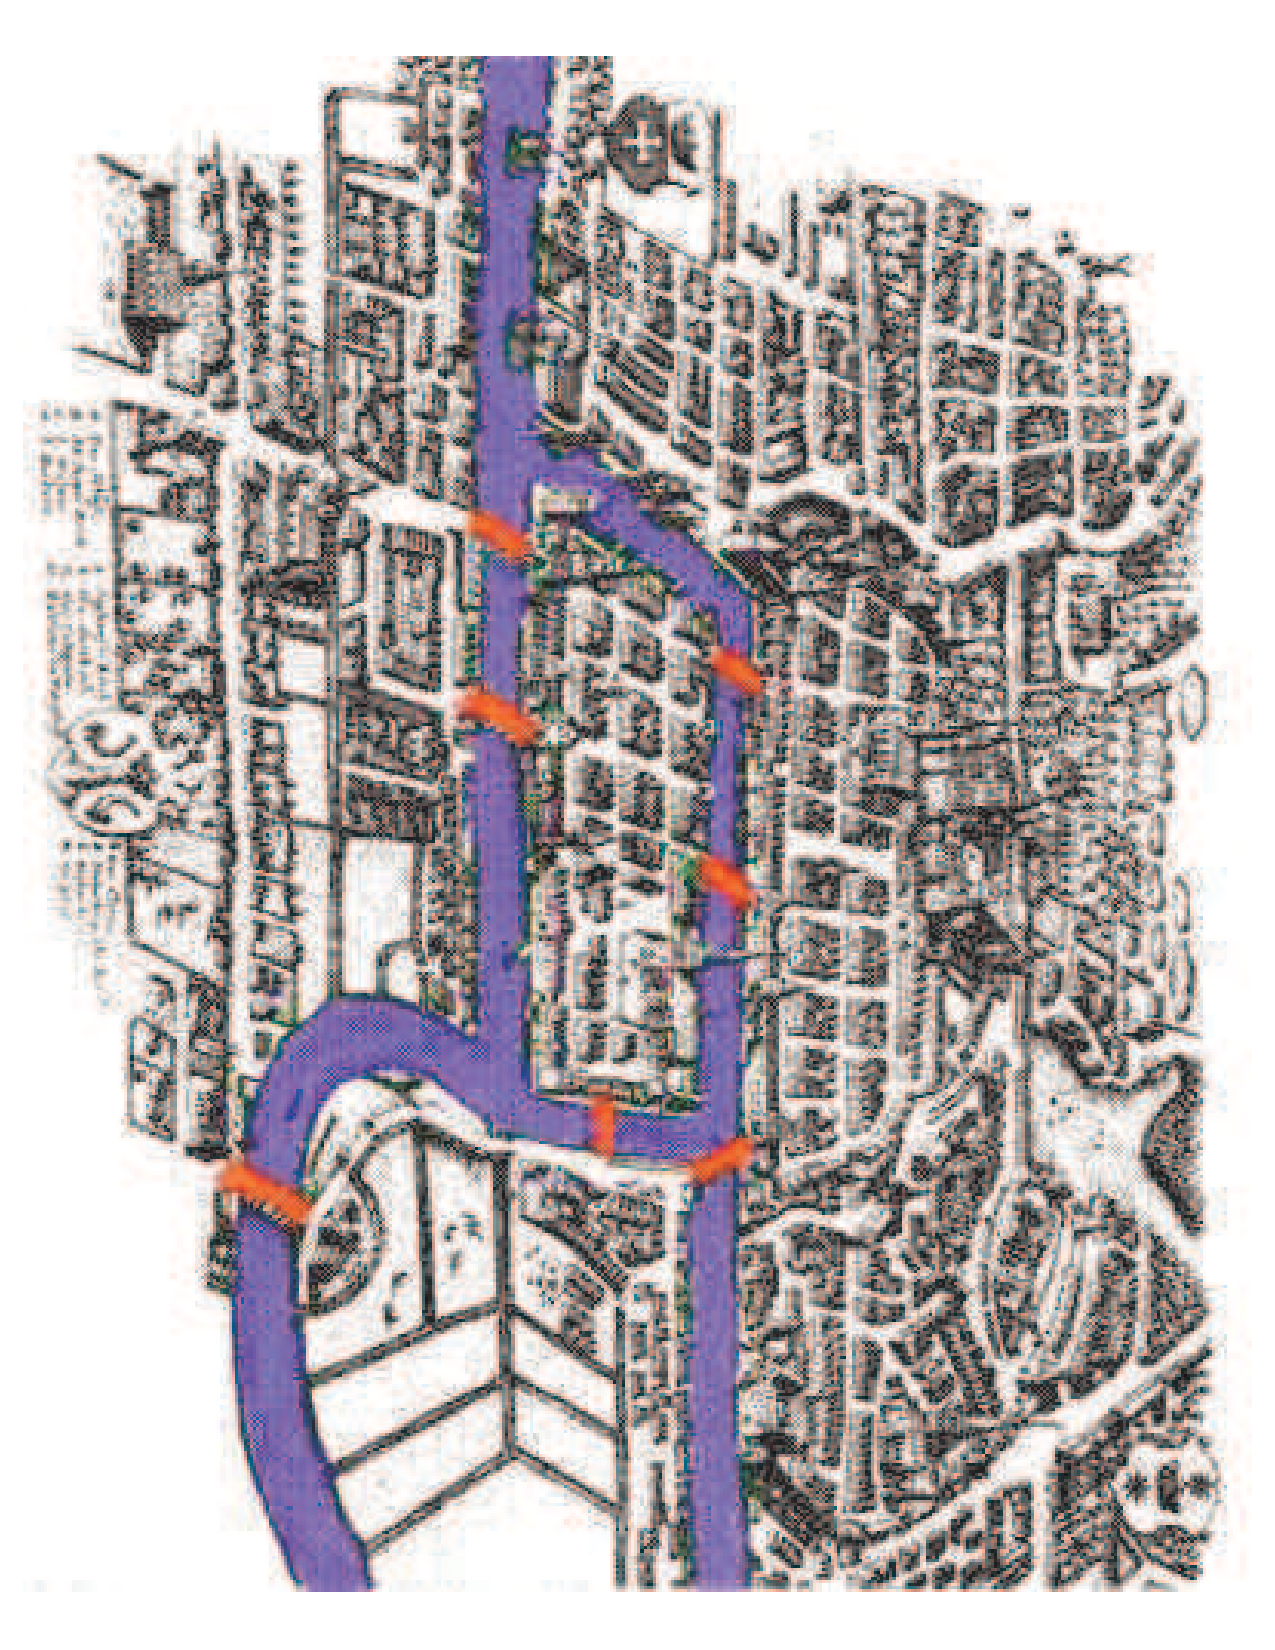
\includegraphics[angle=90,height=.75\textheight]{FIGS_slides/bridge_color}
	\end{center}
\end{frame}

\begin{frame}{The genesis of graphs -- Euler's bridges of K\"onigsberg}
	Cross the 7 bridges in a single walk without recrossing any of them?
	\begin{center}
	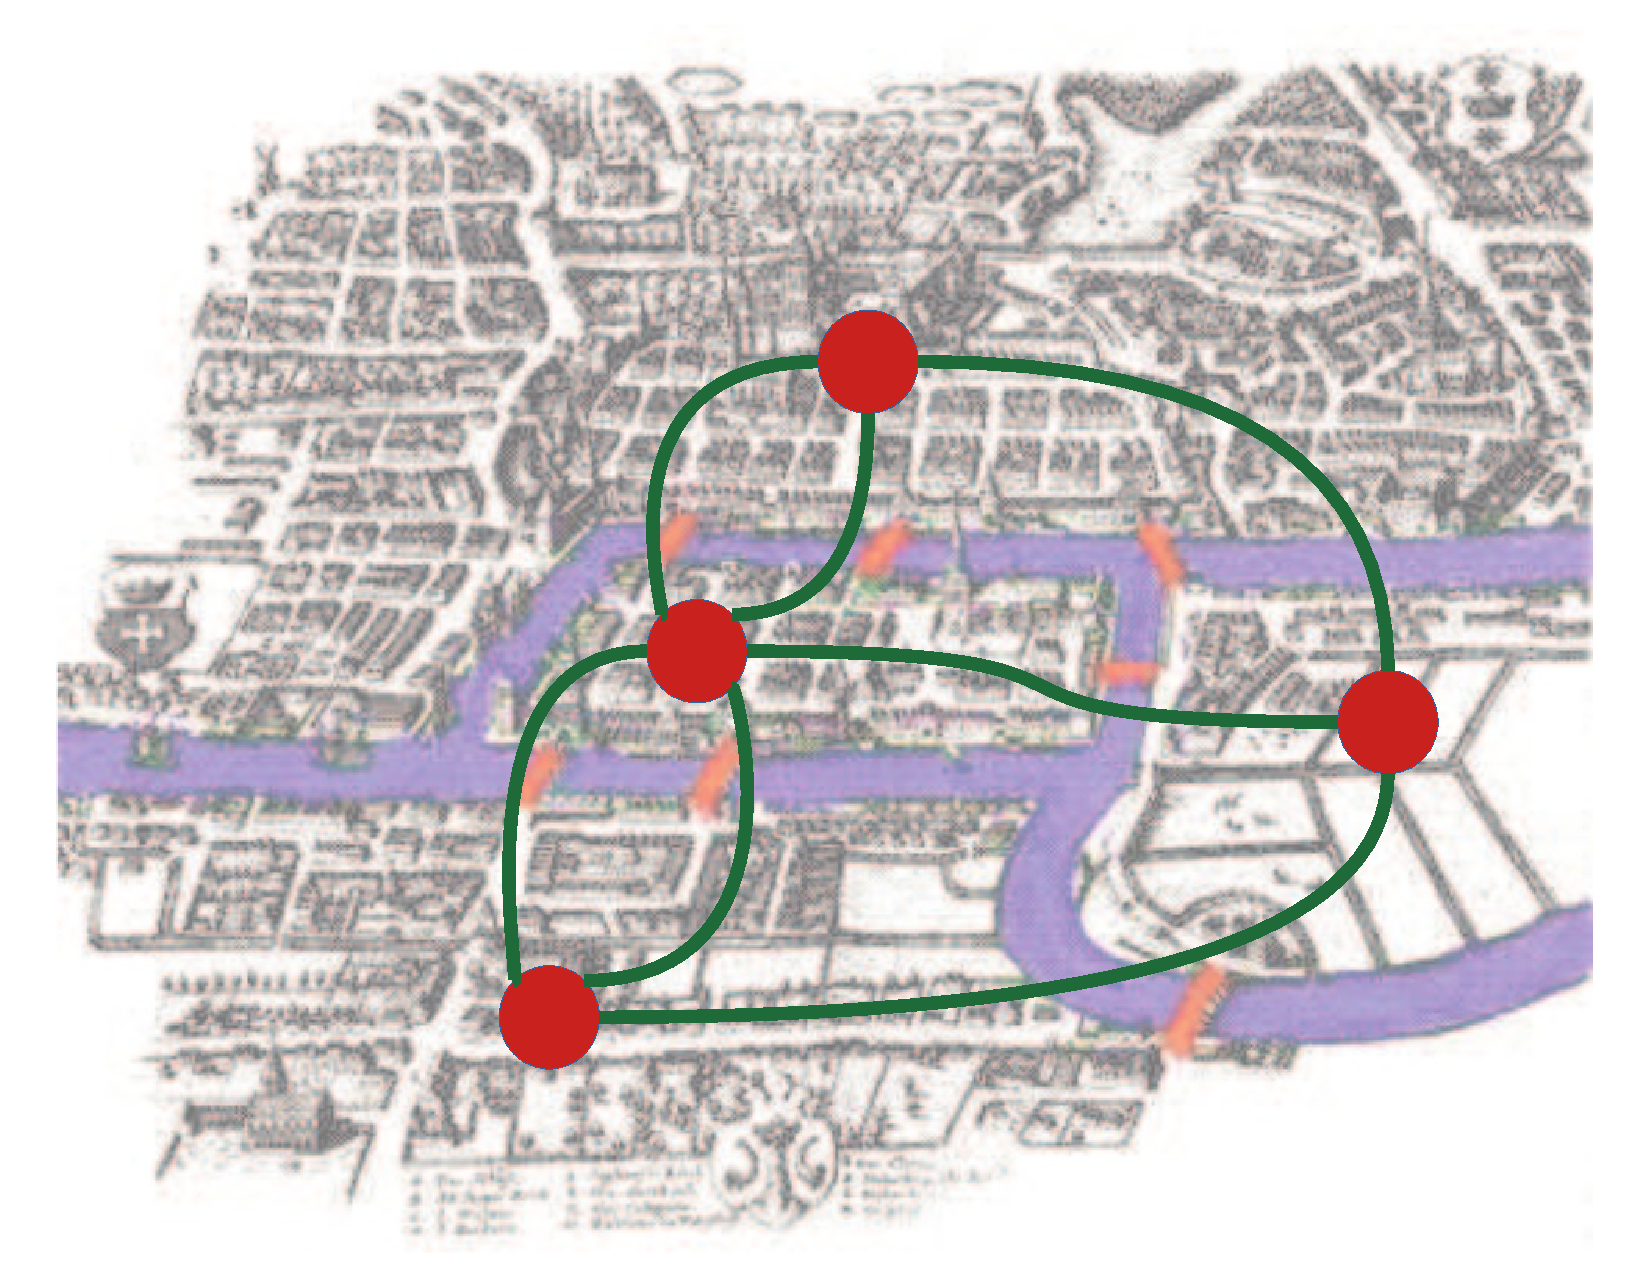
\includegraphics[height=.75\textheight]{FIGS_slides/bridge_color_with_graph}
	\end{center}
\end{frame}

\begin{frame}{The genesis of graphs -- Euler's bridges of K\"onigsberg}
	Cross the 7 bridges in a single walk without recrossing any of them?
	\begin{center}
		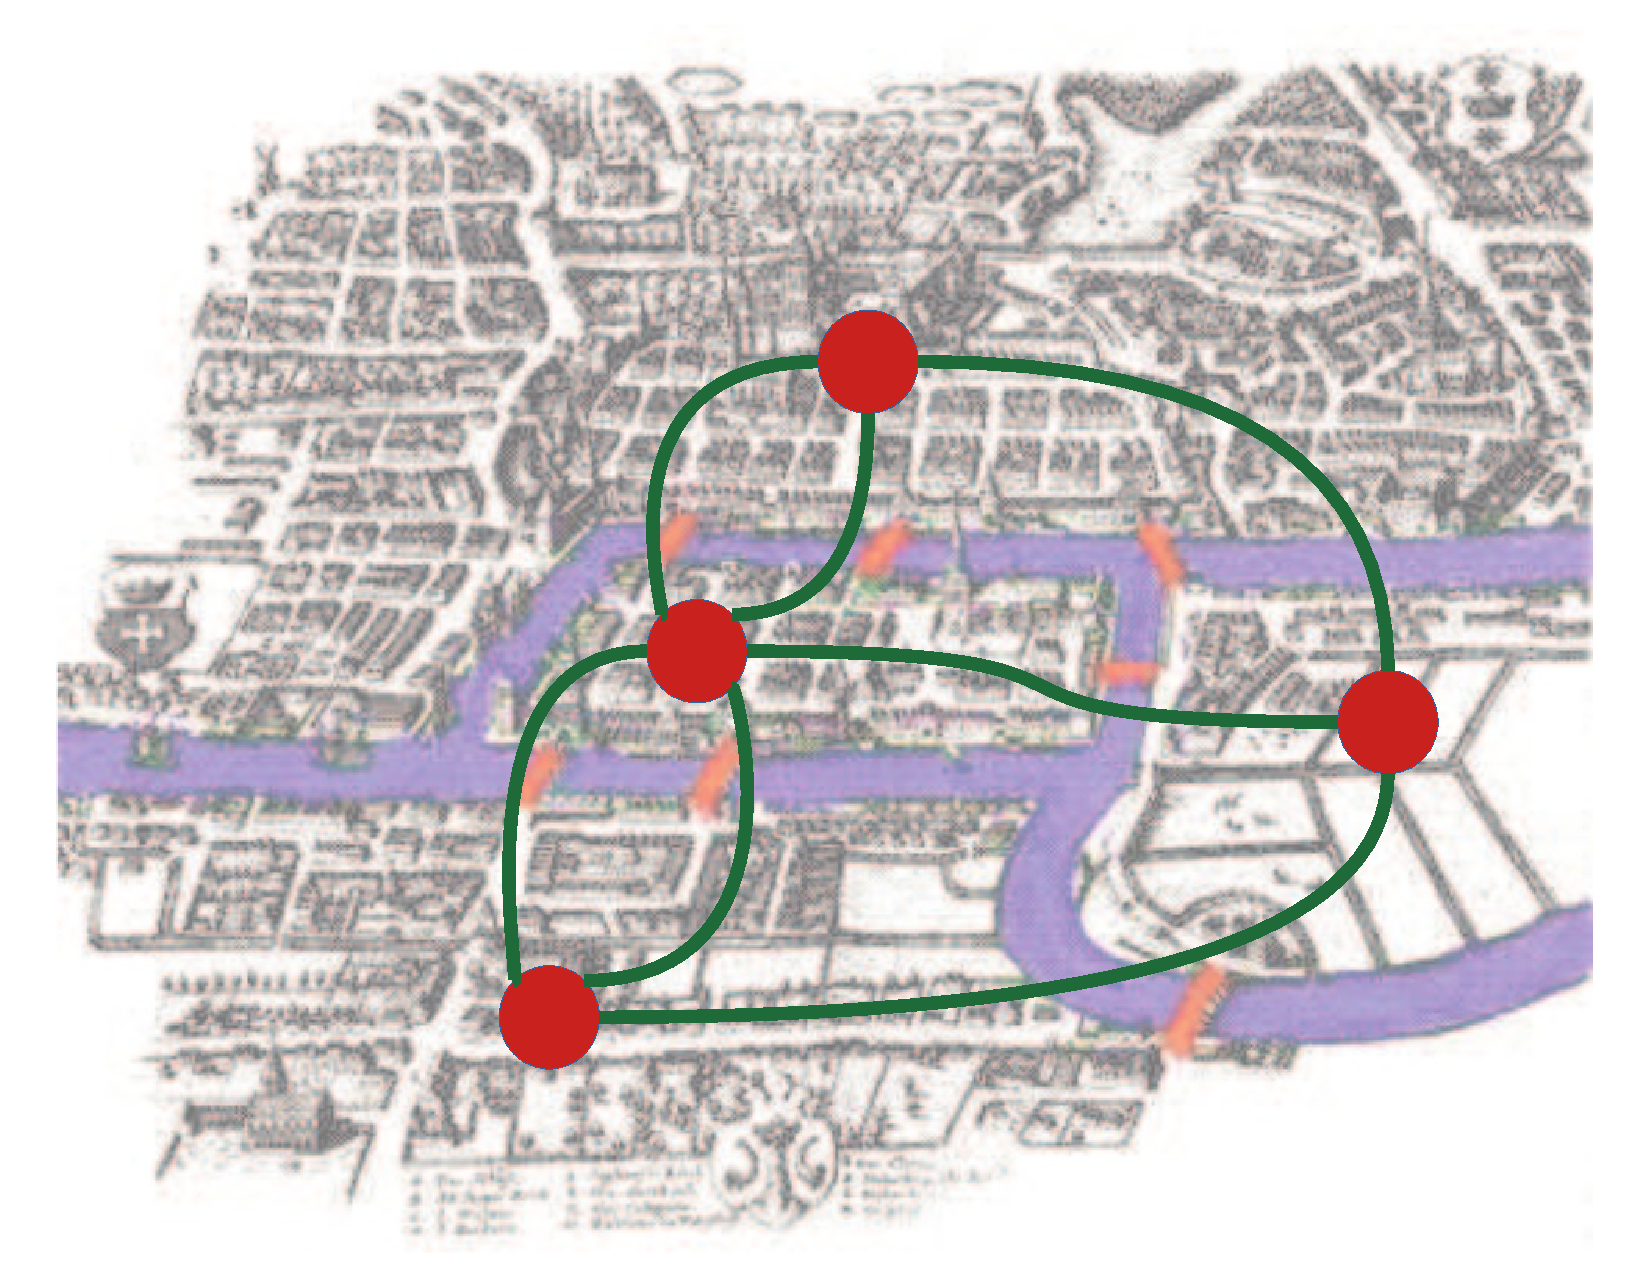
\includegraphics[height=.5\textheight]{FIGS_slides/bridge_color_with_graph}
		\end{center}
	\begin{block}{Mathematical problem}
	Is it possible to find a \emph{trail} containing all \emph{edges} of the graph?
	\end{block}
\end{frame}

\begin{frame}{Finding a cycle with all vertices}
	A salesperson must visit a couple of cities for their job. Is it possible for them to plan a round trip using highways enabling tehm to visit each specified city exactly once?
	\begin{center}
	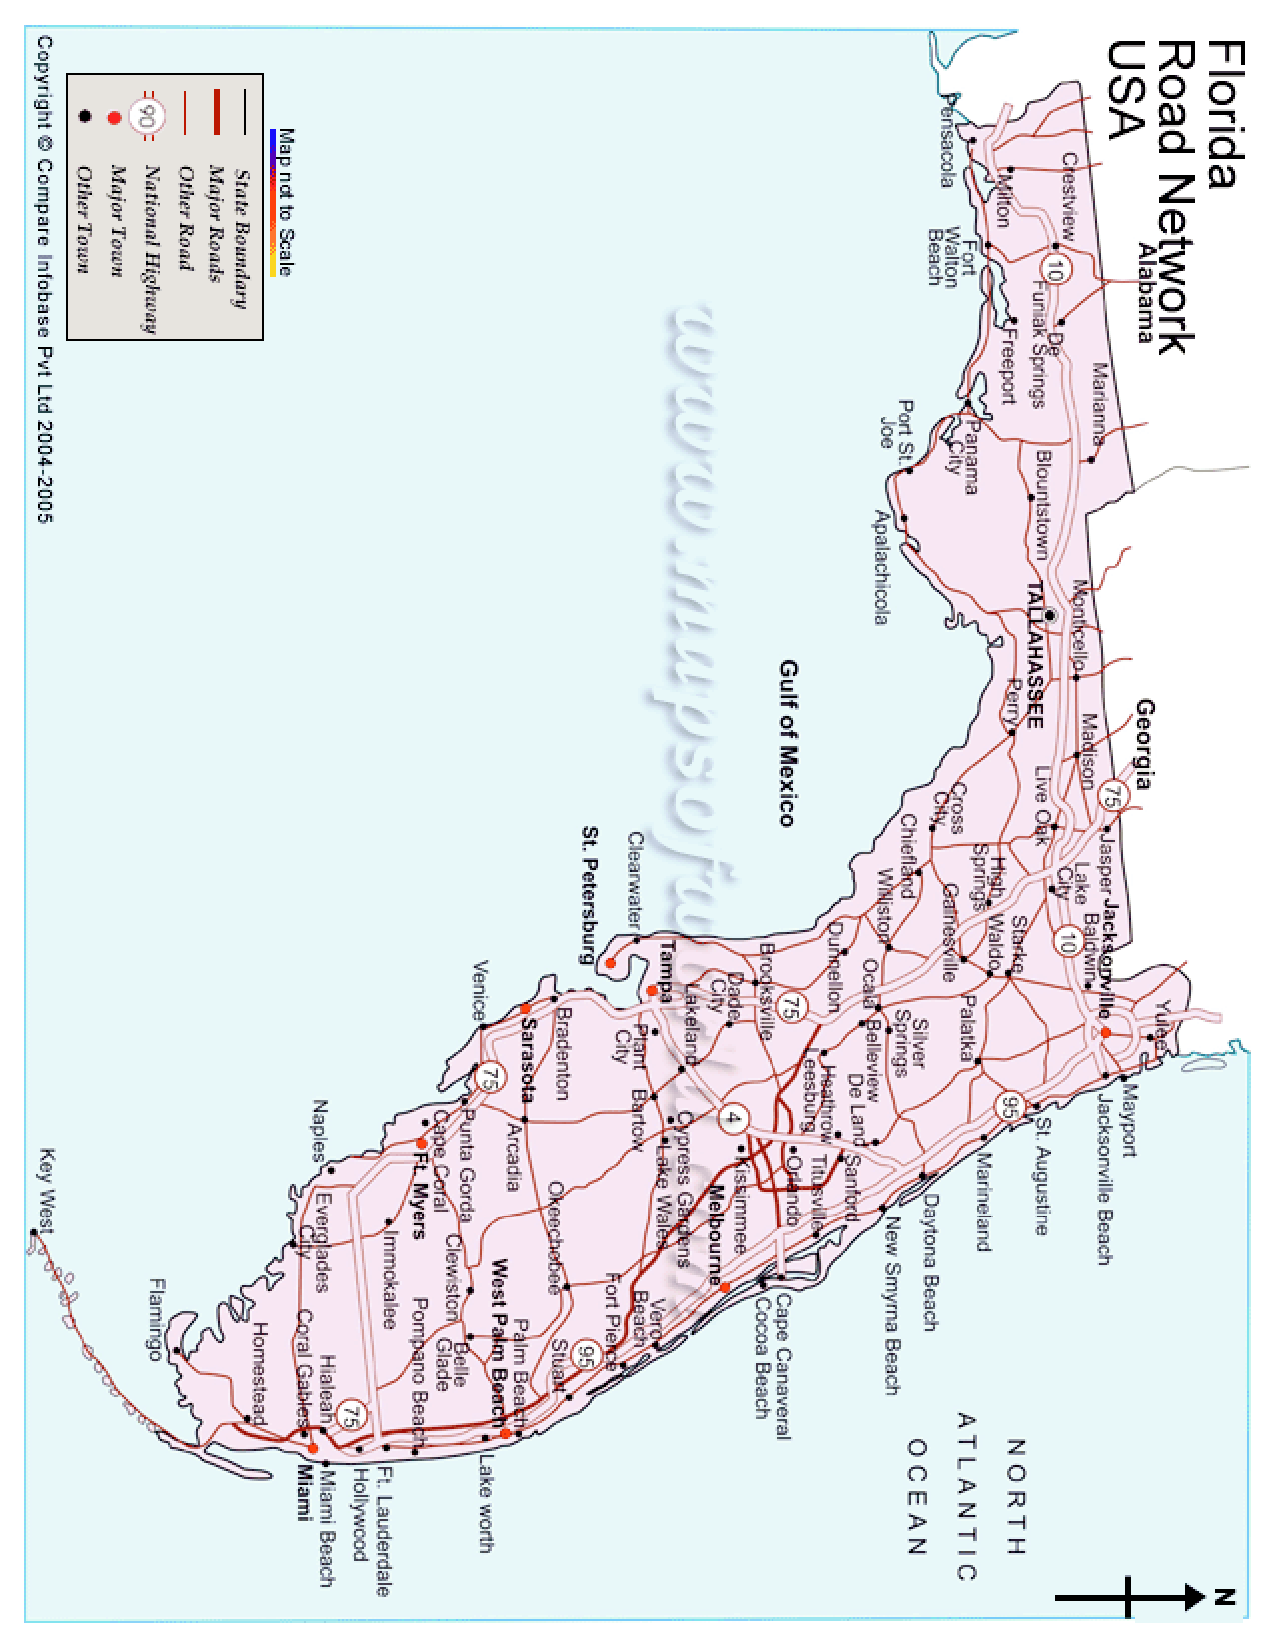
\includegraphics[angle=90,width=.3\textwidth]{FIGS_slides/florida}
	\end{center}
	\begin{itemize}
	\item vertices correspond to cities
	\item two vertices are connected iff a highway connects the corresponding cities and does not pass through any other city.
	\end{itemize}
	\begin{block}{Mathematical problem}
	Is it possible to find a cycle containing all graph vertices?
	\end{block}
\end{frame}

\begin{frame}{How far is it to drive through $n$ cities?}
	What is the minimal length of driving needed to drive through $n$ cities?
	\begin{center}
	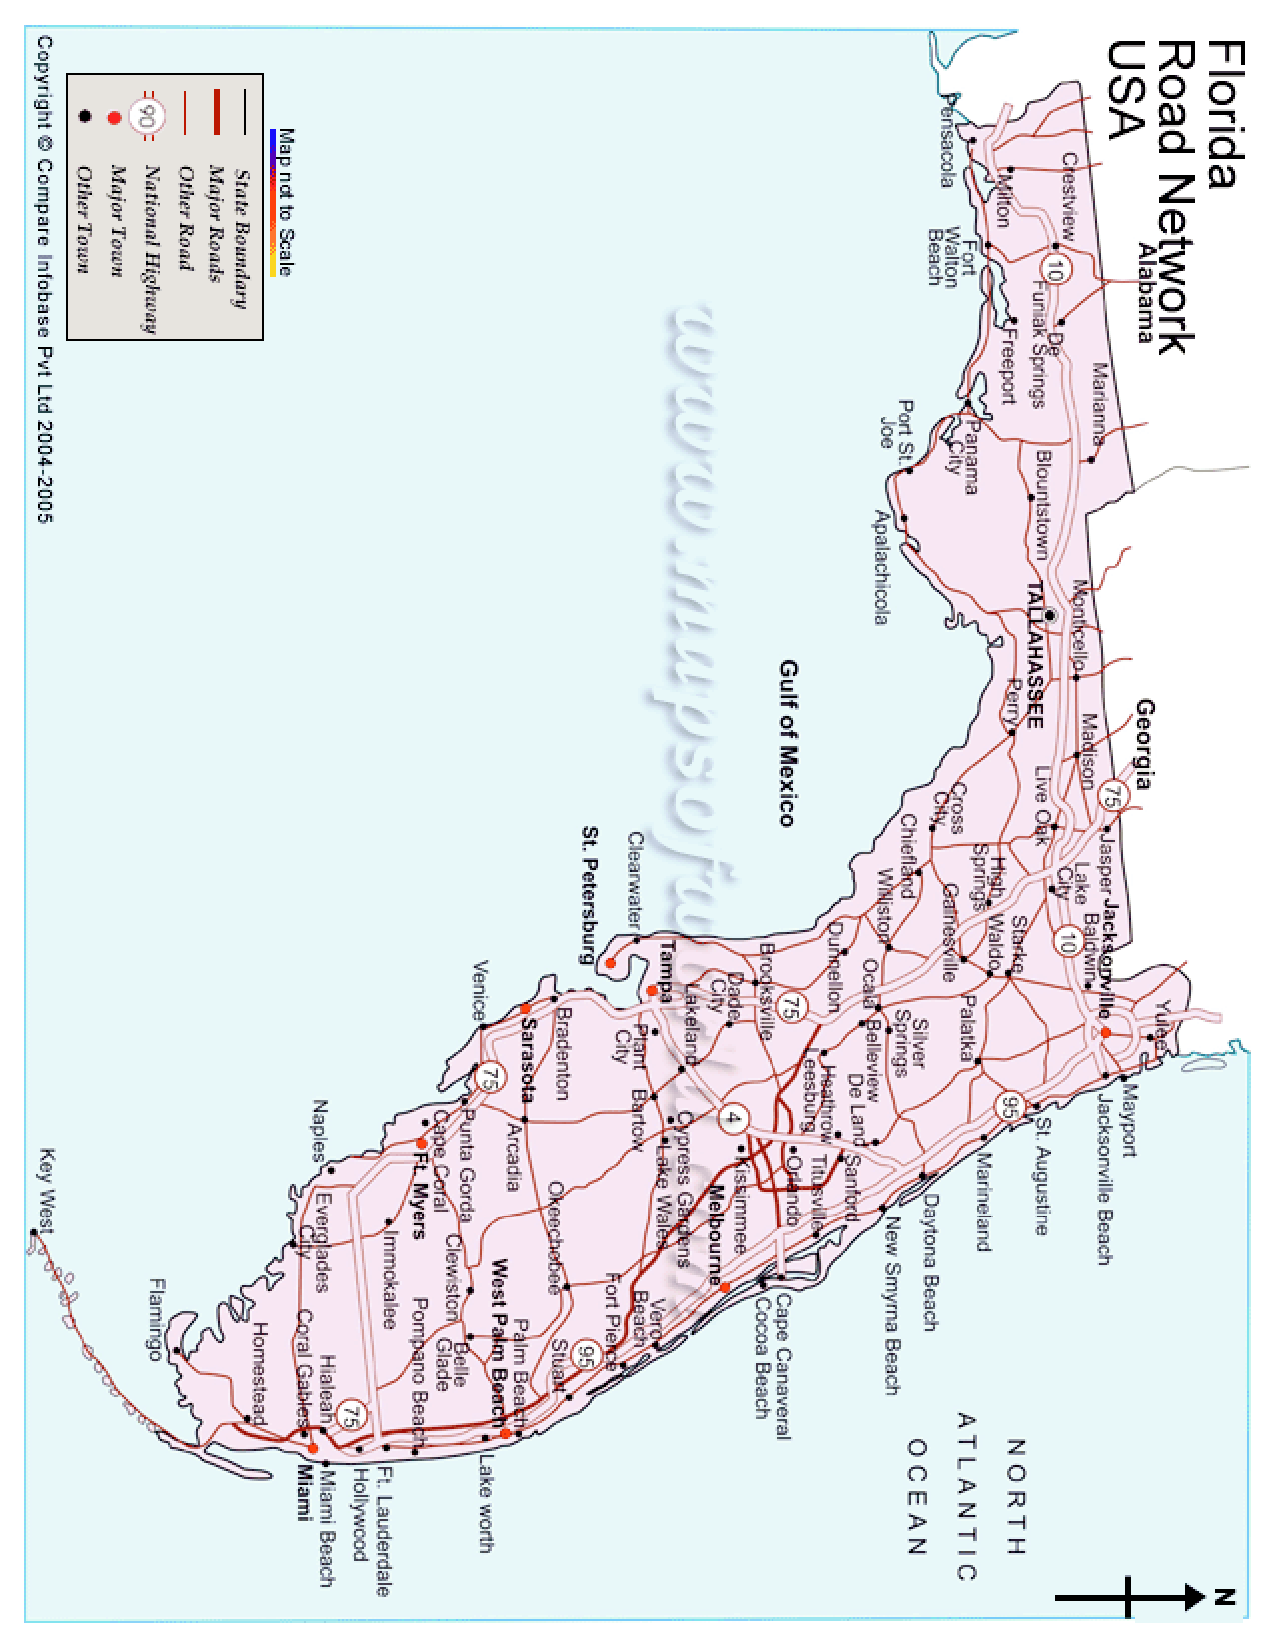
\includegraphics[angle=90,width=.35\textwidth]{FIGS_slides/florida}
	\end{center}
	\begin{itemize}
	\item vertices correspond to the cities
	\item all cities are connected; each edge has a value assigned to it
	\end{itemize}
	\begin{block}{Mathematical problem}
	What is the minimal spanning tree associated to the graph?
	\end{block}
\end{frame}


\begin{frame}{Graphs/networks encode relations}
	Graphs are used in a variety of contexts because they encode \emph{relations} between objects
	\vfill
	Many objects in the world have relations... so graphs are quite easy to find
	\vfill
	We will see many examples later, for now we cover the mathematical background
\end{frame}



\begin{frame}{Graphs vs digraphs vs multigraphs vs multidigraphs vs ...}
	Name-wise and notation-wise, this domain is a bit of a mess
	\vfill
	\begin{itemize}
		\item The vertex set $V$ is essentially the only constant
		\item \emph{Undirected graph} $G=(V,E)$, where $E$ are the \emph{edges}
		\item \emph{Undirected multigraph} $G_M=(V,E)$
		\item \emph{Directed graph} (or \emph{digraph}) $G=(V,A)$, where $A$ are the \emph{arcs}
		\item \emph{Directed multigraph} (or \emph{multidigraph}) $G_M=(V,A)$
		\item Any of the above is called a \emph{graph} and is denoted $G=(V,X)$, when we seek generality
	\end{itemize}
	\vfill
And just to confuse the whole thing more: we often say \emph{graph} for \emph{unoriented graph}
\end{frame}

%%%%%%%%%%%%%%%%%%%%
%%%%%%%%%%%%%%%%%%%%
%%%%%%%%%%%%%%%%%%%%
%%%%%%%%%%%%%%%%%%%%
\section{Binary relations}
\newSectionSlide{FIGS-transitions/Gemini_Generated_Image_fto8nofto8nofto8.jpeg}


\begin{frame}\frametitle{Binary relation}
	\begin{definition}[Binary relation]
	\begin{itemize}
	\item A \defword{binary relation} is an arbitrary association of elements of one set with elements of another (maybe the same) set
	\item  A binary relation over the sets $X$ and $Y$ is defined as a subset of the Cartesian product $X\times Y =\{(x,y)| x\in X , y\in Y\}$
	\item $(x,y)\in R$ is read ``$x$ is $R$-related to $y$'' and is denoted $xRy$
	\item If $(x,y)\not\in R$, we write ``not $x R y$'' or $x\cancel{R} y$
	\end{itemize}
	\end{definition}
\end{frame}
	
\begin{frame}
	\begin{definition}[Properties of binary relations]
		A binary relation $R$ over a set $X$ is
	\begin{itemize}
	\item \defword{Reflexive} if $\forall x\in X$, $xRx$
	\item \defword{Irreflexive} if there does not exist $x\in X$ such that $xRx$
	\item \defword{Symmetric} if $xRy \Rightarrow yRx$
	\item \defword{Asymmetric} if $xRy \Rightarrow $ $y\cancel R x$
	\item \defword{Antisymmetric} if $xRy$ and $yRx$ $\Rightarrow$ $x=y$
	\item \defword{Transitive} if $xRy$ and $yRz$ $\Rightarrow$  $xRz$
	\item \defword{Total} (or \defword{complete}) if $\forall x, y\in X$, $x R y$ or $y R x$
	\end{itemize}
	\end{definition}
\end{frame}
	
	
\begin{frame} 
	\begin{definition}[Equivalence relation]
	 A relation that is reflexive ($\forall x\in X$, $xRx$), symmetric ($xRy \Rightarrow yRx$) and transitive ($xRy$ and $yRz$ $\Rightarrow$  $xRz$) is an \defword{equivalence relation}
	\end{definition}
	\vfill
	\begin{definition}[Partial order]
	 A relation that is reflexive ($\forall x\in X$, $xRx$), antisymmetric ($xRy$ and $yRx$ $\Rightarrow$ $x=y$) and transitive ($xRy$ and $yRz$ $\Rightarrow$  $xRz$) is a \defword{partial order}
	\end{definition}
	\vfill
	\begin{definition}[Total order]
	A partial order that is total ($\forall x, y\in X$, $x R y$ or $y R x$) is a \defword{total order}
	\end{definition}
\end{frame}
	



%%%%%%%%%%%%%%%%%%%%
%%%%%%%%%%%%%%%%%%%%
%%%%%%%%%%%%%%%%%%%%
%%%%%%%%%%%%%%%%%%%%
\section{Undirected graphs}
\newSectionSlide{FIGS-transitions/Gemini_Generated_Image_fto8nofto8nofto8.jpeg}


\begin{frame}\frametitle{The \code{igraph} library}
Throughout these slides, we use the package \code{igraph}
\vfill
I illustrate the functions that can be used to study some of the mathematical notions I introduce
\vfill
I use mostly examples from the \code{igraph} documentation
\end{frame}


\subsection{Undirected graph}
\newSubSectionSlide{FIGS-transitions/Gemini_Generated_Image_fto8nofto8nofto8.jpeg}


\begin{frame}{Graph}
	Intuitively: a graph is a set of points, and a set of relations between the points
	\vfill
	The points are called the \emph{vertices} of the graph and the relations are the \emph{edges} of the graph
	\vfill
	We can also think of the relations as being one directional, in which case the relations are the \emph{arcs} of the digraph (a contraction of ``directed graph'')
\end{frame}


\begin{frame}\frametitle{Graph, vertex and edge} 
	\begin{definition}[Graph]
	An \defword{undirected graph} is a pair $G=(V,E)$ of sets such that
	\begin{itemize}
	\item $V$ is a set of points:  $V=\{v_1,\ldots,v_p\}$
	\item $E$ is a set of 2-element subsets of $V$: $E=\{\{v_i,v_j\},\{v_i,v_k\},\ldots,\{v_n,v_p\}\}$ or $E=\{v_iv_j,v_iv_k,\ldots,v_nv_p\}$
	\end{itemize}
	\end{definition}
	\begin{definition}[Vertex]
	The elements of $V$ are the \defword{vertices} (or nodes, or points) of the graph $G$.
	$V$ (or $V(G)$) is the vertex set of the graph $G$
	\end{definition}
	\begin{definition}[Edge]
	The elements of $E$ are the \defword{edges} (or lines) of the graph $G$.
	$E$ (or $E(G)$) is the edge set of the graph $G$
	\end{definition}
\end{frame}


\begin{frame}[fragile]\frametitle{Setting up graphs in \code{igraph}}
\begin{knitrout}
\definecolor{shadecolor}{rgb}{0.969, 0.969, 0.969}\color{fgcolor}\begin{kframe}
\begin{alltt}
\hldef{G} \hlkwb{<-} \hlkwd{make_empty_graph}\hldef{()}
\hldef{G} \hlkwb{<-} \hlkwd{make_graph}\hldef{(}\hlkwc{edges} \hldef{=} \hlkwd{c}\hldef{(}\hlnum{1}\hldef{,} \hlnum{2}\hldef{,} \hlnum{1}\hldef{,} \hlnum{5}\hldef{),} \hlkwc{n} \hldef{=} \hlnum{10}\hldef{,}
                \hlkwc{directed} \hldef{=} \hlnum{FALSE}\hldef{)}
\hldef{G} \hlkwb{<-} \hlkwd{make_graph}\hldef{(}\hlsng{"Zachary"}\hldef{)}
\hlkwd{plot}\hldef{(G,} \hlkwc{main} \hldef{=} \hlsng{"Data on a Karate club"}\hldef{)}
\end{alltt}
\end{kframe}
\end{knitrout}
\end{frame}

\maxFrameImage{FIGS/graphs-setup-graph-1-1.pdf}

\begin{frame}\frametitle{Order and Size}
	\begin{definition}[Order of a graph]
	The number of vertices in $G$ is the \defword{order} of $G$. Using the notation $|V(G)|$ for the \emph{cardinality} of $V(G)$,
	$$|V(G)|=\textrm{order of G}$$
	\end{definition}
	\vfill
	\begin{definition}[Size of a graph]
	The number of edges in $G$ is the \defword{size} of $G$,
	$$|E(G)|=\textrm{size of G}$$
	\end{definition}
	\vfill
	\begin{itemize}
	\item A graph having order $p$ and size $q$ is called a $(p,q)-$graph
	\item A graph is finite if $|V(G)|<\infty$
	\end{itemize}
\end{frame}

\begin{frame}[fragile]\frametitle{Some simple measures}
\begin{knitrout}
\definecolor{shadecolor}{rgb}{0.969, 0.969, 0.969}\color{fgcolor}\begin{kframe}
\begin{alltt}
\hlkwd{V}\hldef{(G)}
\end{alltt}
\begin{verbatim}
## + 34/34 vertices, from c9db94e:
##  [1]  1  2  3  4  5  6  7  8  9 10 11 12 13 14 15 16 17 18 19 20 21 22 23 24 25
## [26] 26 27 28 29 30 31 32 33 34
\end{verbatim}
\begin{alltt}
\hlkwd{head}\hldef{(}\hlkwd{E}\hldef{(G))}
\end{alltt}
\begin{verbatim}
## + 6/78 edges from c9db94e:
## [1] 1--2 1--3 1--4 1--5 1--6 1--7
\end{verbatim}
\begin{alltt}
\hlkwd{gorder}\hldef{(G)}
\end{alltt}
\begin{verbatim}
## [1] 34
\end{verbatim}
\begin{alltt}
\hlkwd{gsize}\hldef{(G)}
\end{alltt}
\begin{verbatim}
## [1] 78
\end{verbatim}
\end{kframe}
\end{knitrout}
\end{frame}

\begin{frame}\frametitle{Incident -- Adjacent}
	\begin{definition}[Incident]
	\begin{itemize}
	\item A vertex $v$ is \defword{incident} with an edge $e$ if $v\in e$; then $e$ is an edge at $v$
	\item If $e=uv\in E(G)$, then $u$ and $v$ are each incident with $e$
	\item The two vertices incident with an edge are its ends
	\item An edge $e=uv$ is incident with both vertices $u$ and $v$
	\end{itemize}
	\end{definition}
	\vfill
	\begin{definition}[Adjacent]
	\begin{itemize}
	\item Two vertices $u$ and $v$ are \defword{adjacent} in a graph $G$ if $uv\in E(G)$
	\item If $uv$ and $uw$ are distinct edges (i.e. $v\not=w$) of a graph $G$, then $uv$ and $uw$ are adjacent edges
	\end{itemize}
	\end{definition}
\end{frame}


\begin{frame}[fragile]\frametitle{Incident vertices}
\begin{knitrout}
\definecolor{shadecolor}{rgb}{0.969, 0.969, 0.969}\color{fgcolor}\begin{kframe}
\begin{alltt}
\hlkwd{incident}\hldef{(G,} \hlnum{1}\hldef{)}
\end{alltt}
\begin{verbatim}
## + 16/78 edges from c9db94e:
##  [1] 1-- 2 1-- 3 1-- 4 1-- 5 1-- 6 1-- 7 1-- 8 1-- 9 1--11 1--12 1--13 1--14
## [13] 1--18 1--20 1--22 1--32
\end{verbatim}
\begin{alltt}
\hlkwd{incident_edges}\hldef{(G,} \hlkwd{c}\hldef{(}\hlnum{1}\hldef{,} \hlnum{2}\hldef{))}
\end{alltt}
\begin{verbatim}
## [[1]]
## + 16/78 edges from c9db94e:
##  [1] 1-- 2 1-- 3 1-- 4 1-- 5 1-- 6 1-- 7 1-- 8 1-- 9 1--11 1--12 1--13 1--14
## [13] 1--18 1--20 1--22 1--32
## 
## [[2]]
## + 9/78 edges from c9db94e:
## [1] 1-- 2 2-- 3 2-- 4 2-- 8 2--14 2--18 2--20 2--22 2--31
\end{verbatim}
\end{kframe}
\end{knitrout}
\end{frame}

\begin{frame}[fragile]\frametitle{Adjacent vertices}
\begin{knitrout}
\definecolor{shadecolor}{rgb}{0.969, 0.969, 0.969}\color{fgcolor}\begin{kframe}
\begin{alltt}
\hlkwd{adjacent_vertices}\hldef{(G,} \hlkwc{v} \hldef{=} \hlnum{1}\hldef{)}
\end{alltt}
\begin{verbatim}
## [[1]]
## + 16/34 vertices, from c9db94e:
##  [1]  2  3  4  5  6  7  8  9 11 12 13 14 18 20 22 32
\end{verbatim}
\begin{alltt}
\hlkwd{adjacent_vertices}\hldef{(G,} \hlkwc{v} \hldef{=} \hlkwd{c}\hldef{(}\hlnum{1}\hldef{,} \hlnum{2}\hldef{))}
\end{alltt}
\begin{verbatim}
## [[1]]
## + 16/34 vertices, from c9db94e:
##  [1]  2  3  4  5  6  7  8  9 11 12 13 14 18 20 22 32
## 
## [[2]]
## + 9/34 vertices, from c9db94e:
## [1]  1  3  4  8 14 18 20 22 31
\end{verbatim}
\end{kframe}
\end{knitrout}
\end{frame}


\begin{frame}
	\begin{definition}[Multiple edge]
	\defword{Multiple edges} are two or more edges connecting the same two vertices within a multigraph
	\end{definition}
	\vfill
	\begin{definition}[Loop]
	A \defword{loop} is an edge with both the same ends; \emph{e.g.} $\{u,u\}$ is a loop
	\end{definition}
	\vfill
	\begin{definition}[Simple graph]
		A \defword{simple graph} is a graph which contains no loops or multiple edges
	\end{definition}
	\vfill
	\begin{definition}[Multigraph]
		A \defword{multigraph} is a graph which can contain multiple edges or loops
	\end{definition}
\end{frame}


\begin{frame}[fragile]\frametitle{Testing for these properties}
\begin{knitrout}
\definecolor{shadecolor}{rgb}{0.969, 0.969, 0.969}\color{fgcolor}\begin{kframe}
\begin{alltt}
\hlkwd{any_multiple}\hldef{(G)}
\end{alltt}
\begin{verbatim}
## [1] FALSE
\end{verbatim}
\begin{alltt}
\hlkwd{any_loop}\hldef{(G)}
\end{alltt}
\begin{verbatim}
## [1] FALSE
\end{verbatim}
\begin{alltt}
\hlkwd{is_simple}\hldef{(G)}
\end{alltt}
\begin{verbatim}
## [1] TRUE
\end{verbatim}
\end{kframe}
\end{knitrout}
\end{frame}



\begin{frame}\frametitle{Graph and binary relations}
A simple graph $G$ can be defined in term of a vertex set $V$ and a binary relation over $V$ that is
	\begin{itemize}
		\item irreflexive ($\forall u\in V$, $u\cancel Ru$)
		\item symmetric ($\forall u,v\in V$, $uRv\implies vRu$)
	\end{itemize}
	\vfill
	The set of edges $E(G)$ is the set of symmetric pairs in $R$
	\vfill
	If $R$ is not irreflexive, the graph is not simple
\end{frame}


\subsection{Degree of a vertex}
\newSubSectionSlide{FIGS-transitions/Gemini_Generated_Image_fto8nofto8nofto8.jpeg}

\begin{frame}
	\begin{definition}[Degree of a vertex]
	Let $v$ be a vertex of $G=(V,E)$.
	\begin{itemize}
	\item The number of edges of $G$ incident with $v$ is the \defword{degree} of $v$ in $G$
	\item The number of edges of $G$ at $v$ is the \defword{degree} of $v$ in $G$
	\item The degree of $v$ in $G$ is noted $d_G(v)$ or $deg_G(v)$
	\end{itemize}
	\end{definition}
	\vfill
	\begin{theorem}\label{th:sum-degrees}
	Let $G$ be a $(p,q)-$graph with vertices $v_1$, $\dots$, $v_p$, then
	\[
		\sum_{i=1}^{p}d_G(v_i)=2q
	\]
	\end{theorem}
\end{frame}

\begin{frame}[fragile]\frametitle{Degree}
\begin{knitrout}
\definecolor{shadecolor}{rgb}{0.969, 0.969, 0.969}\color{fgcolor}\begin{kframe}
\begin{alltt}
\hlkwd{degree}\hldef{(G)}
\end{alltt}
\begin{verbatim}
##  [1] 16  9 10  6  3  4  4  4  5  2  3  1  2  5  2  2  2  2  2  3  2  2  2  5  3
## [26]  3  2  4  3  4  4  6 12 17
\end{verbatim}
\begin{alltt}
\hlkwd{degree_distribution}\hldef{(G)}
\end{alltt}
\begin{verbatim}
##  [1] 0.00000000 0.02941176 0.32352941 0.17647059 0.17647059 0.08823529
##  [7] 0.05882353 0.00000000 0.00000000 0.02941176 0.02941176 0.00000000
## [13] 0.02941176 0.00000000 0.00000000 0.00000000 0.02941176 0.02941176
\end{verbatim}
\begin{alltt}
\hlkwd{plot}\hldef{(}\hlkwd{degree_distribution}\hldef{(G),}
     \hlkwc{type} \hldef{=} \hlsng{"b"}\hldef{,}
     \hlkwc{xlab} \hldef{=} \hlsng{"Degree"}\hldef{,} \hlkwc{ylab} \hldef{=} \hlsng{"Frequency"}\hldef{,}
     \hlkwc{main} \hldef{=} \hlsng{"Degree distribution of the Karate graph"}\hldef{)}
\end{alltt}
\end{kframe}
\end{knitrout}
\end{frame}

\maxFrameImage{FIGS/graphs-vertex-degrees-undirected-1.pdf}



\begin{frame}
\begin{definition}[{Odd vertex}]
A vertex is an \defword{odd vertex} is its degree is odd
\end{definition}
\vfill
\begin{definition}[{Even vertex}]
A vertex is called \defword{even vertex} is its degree is even
\end{definition}
\vfill
\begin{theorem}\label{th:even-nb-odd-vertices}
Every graph contains an even number of odd vertices
\end{theorem}
\end{frame}

\begin{frame}[fragile]\frametitle{Illustration of recent results}
Theorem~\ref{th:sum-degrees} states that a $(p,q)-$graph has $\sum_{i=1}^{p}d_G(v_i)=2q$
\begin{knitrout}
\definecolor{shadecolor}{rgb}{0.969, 0.969, 0.969}\color{fgcolor}\begin{kframe}
\begin{alltt}
\hlkwd{sum}\hldef{(}\hlkwd{degree}\hldef{(G))} \hlopt{==} \hlnum{2}\hlopt{*}\hlkwd{length}\hldef{(}\hlkwd{E}\hldef{(G))}
\end{alltt}
\begin{verbatim}
## [1] TRUE
\end{verbatim}
\end{kframe}
\end{knitrout}
\vfill
Theorem~\ref{th:even-nb-odd-vertices} states that every graph contains an even number of odd vertices
\begin{knitrout}
\definecolor{shadecolor}{rgb}{0.969, 0.969, 0.969}\color{fgcolor}\begin{kframe}
\begin{alltt}
\hlkwd{sum}\hldef{(pracma}\hlopt{::}\hlkwd{mod}\hldef{(}\hlkwd{degree}\hldef{(G),}\hlnum{2}\hldef{))}
\end{alltt}
\begin{verbatim}
## [1] 12
\end{verbatim}
\end{kframe}
\end{knitrout}
(\code{mode(x,2)} returns 1 if $x$ is odd so \code{sum} counts how many are odd)
\end{frame}

\begin{frame}[fragile]{Regular graph}
\begin{definition}[{Regular graph}]
	If all the vertices of $G$ have the same degree $k$, then the graph $G$ is $k$-regular
\end{definition}
\vfill
\begin{knitrout}
\definecolor{shadecolor}{rgb}{0.969, 0.969, 0.969}\color{fgcolor}\begin{kframe}
\begin{alltt}
\hlkwd{length}\hldef{(}\hlkwd{unique}\hldef{(}\hlkwd{degree}\hldef{(G)))} \hlopt{==} \hlnum{1}
\end{alltt}
\begin{verbatim}
## [1] FALSE
\end{verbatim}
\end{kframe}
\end{knitrout}
\end{frame}




%%%%%%%%%%%%%%%%%%%%%%%
%%%%%%%%%%%%%%%%%%%%%%%
\subsection{Isomorphic graphs}
\newSubSectionSlide{FIGS-transitions/Gemini_Generated_Image_fto8nofto8nofto8.jpeg}

\begin{frame} \frametitle{Isomorphic graphs} 
\begin{definition}[Isomorphic graphs]
Let $G_1=(V(G_1),E(G_1))$ and $G_2=(V(G_2),E(G_2))$ be two graphs.
$G_1$ and $G_2$ are \defword{isomorphic} if there exists an isomorphism $\phi$ from $G_1$ to $G_2$, that is defined as an injective mapping $\phi:\; V(G_1) \rightarrow V(G_2)$ such that two vertices $u_1$ and $v_1$ are adjacent in $G_1$ $\iff$ the vertices $\phi(u_1)$ and $\phi(v_1)$ are adjacent in $G_2$
\end{definition}
\end{frame}
 
 
 
\begin{frame}
If $\phi$ is an isomorphism from $G_1$ to $G_2$, then the inverse mapping $\phi ^{-1}$ from $V(G_2)$ to $V(G_1)$ also satisfies the definition of an isomorphism.
As a consequence, if $G_1$ and $G_2$ are isomorphic graphs, then
\begin{itemize}
\item $G_1$ is isomorphic to $G_2$
\item $G_2$ is isomorphic to $G_1$
\end{itemize}
\vfill
\begin{theorem}
The relation ``is isomorphic to'' is an equivalence relation on the set of all graphs
\end{theorem}
\vfill
\begin{theorem}
If $G_1$ and $G_2$ are isomorphic graphs, then the degrees of vertices of $G_1$ are exactly the degrees of vertices of $G_2$
\end{theorem}
\end{frame}

\begin{frame}[fragile]\frametitle{Testing isomorphicity}
Create two isomorphic graphs by permuting the vertices of the first, then test if they are isomorphic
\vfill
\begin{knitrout}
\definecolor{shadecolor}{rgb}{0.969, 0.969, 0.969}\color{fgcolor}\begin{kframe}
\begin{alltt}
\hldef{g1} \hlkwb{<-} \hlkwd{sample_pa}\hldef{(}\hlnum{30}\hldef{,} \hlkwc{m} \hldef{=} \hlnum{2}\hldef{,} \hlkwc{directed} \hldef{=} \hlnum{FALSE}\hldef{)}
\hldef{g2} \hlkwb{<-} \hlkwd{permute}\hldef{(g1,} \hlkwd{sample}\hldef{(}\hlkwd{vcount}\hldef{(g1)))}
\hlcom{# should be TRUE}
\hlkwd{isomorphic}\hldef{(g1, g2)}
\end{alltt}
\begin{verbatim}
## [1] TRUE
\end{verbatim}
\end{kframe}
\end{knitrout}
\end{frame}


%%%%%%%%%%%%%%%%%%%%%%%
%%%%%%%%%%%%%%%%%%%%%%%
\subsection{Subgraphs, unions of graphs}
\newSubSectionSlide{FIGS-transitions/Gemini_Generated_Image_fto8nofto8nofto8.jpeg}

\begin{frame}\frametitle{Subgraph}
\begin{definition}[Subgraph]
Let $G=(V,E)$ be a graph.
A graph $H=(V(H),E(H))$ is a \defword{subgraph} of $G$ if $V(H)\subseteq V$ and $E(H)\subseteq E$
\end{definition}
\end{frame}

\begin{frame}[fragile]\frametitle{Extracting a subgraph}
\begin{knitrout}
\definecolor{shadecolor}{rgb}{0.969, 0.969, 0.969}\color{fgcolor}\begin{kframe}
\begin{alltt}
\hldef{G_sub} \hlkwb{=} \hlkwd{induced_subgraph}\hldef{(G,} \hlkwd{c}\hldef{(}\hlnum{1}\hlopt{:}\hlnum{5}\hldef{,} \hlnum{11}\hlopt{:}\hlnum{14}\hldef{))}
\hlkwd{plot}\hldef{(G_sub,} \hlkwc{main} \hldef{=} \hlsng{"A subgraph of the Karate graph"}\hldef{)}
\end{alltt}
\end{kframe}
\end{knitrout}
\end{frame}

\maxFrameImage{FIGS/graphs-extract-subgraph-1.pdf}

\begin{frame}[fragile]\frametitle{Naming vertices}
Note that vertices (and as a consequence, edges) will be relabelled, so \code{G\_sub} has vertices labelled 1 to 9
\vfill
You can name vertices if you want to avoid this
\begin{knitrout}
\definecolor{shadecolor}{rgb}{0.969, 0.969, 0.969}\color{fgcolor}\begin{kframe}
\begin{alltt}
\hlkwd{V}\hldef{(G)}\hlopt{$}\hldef{name} \hlkwb{=} \hlnum{1}\hlopt{:}\hlkwd{length}\hldef{(}\hlkwd{V}\hldef{(G))}
\hldef{G_sub} \hlkwb{=} \hlkwd{induced_subgraph}\hldef{(G,} \hlkwd{c}\hldef{(}\hlnum{1}\hlopt{:}\hlnum{5}\hldef{,} \hlnum{11}\hlopt{:}\hlnum{14}\hldef{))}
\hlkwd{plot}\hldef{(G_sub,} \hlkwc{labels} \hldef{=} \hlkwd{V}\hldef{(G)}\hlopt{$}\hldef{name,}
     \hlkwc{main} \hldef{=} \hlsng{"Subgraph of the Karate graph preserving names"}\hldef{)}
\end{alltt}
\end{kframe}
\end{knitrout}
\end{frame}

\maxFrameImage{FIGS/graphs-subgraph-named-vertices-1.pdf}


\begin{frame}
Let $G_1=(V_1,E_1)$ and $G_2=(V_2,E_2)$ be two graphs
\begin{definition}[{Union of $G_1$ and $G_2$}]
$G_1\cup G_2=(V_1\cup V_2,E_1\cup E_2)$
\end{definition}
\begin{definition}[{Intersection of $G_1$ and $G_2$}]
$G_1\cap G_2=(V_1\cap V_2,E_1\cap E_2)$
\end{definition}
\begin{definition}[{Disjoint graphs}]
If $G_1\cap G_2=(\emptyset,\emptyset)= \emptyset$ (empty graph) then $G_1$ and $G_2$ are \defword{disjoint}
\end{definition}
\begin{definition}[{Complement of $G_1$}]
The \defword{complement} $\bar G_1$ of $G_1$ is the graph on $V_1$, with the edge set $E(\bar G_1)=[V_1]^2\backslash E_1$ ($e\in E(\bar G_1)$ $\iff$ $e\not \in E_1$)
\end{definition}
\end{frame}


\begin{frame}[fragile]\frametitle{Union}
\begin{knitrout}
\definecolor{shadecolor}{rgb}{0.969, 0.969, 0.969}\color{fgcolor}\begin{kframe}
\begin{alltt}
\hldef{net1} \hlkwb{<-} \hlkwd{graph_from_literal}\hldef{(}
  \hldef{D} \hlopt{-} \hldef{A}\hlopt{:}\hldef{B}\hlopt{:}\hldef{F}\hlopt{:}\hldef{G, A} \hlopt{-} \hldef{C} \hlopt{-} \hldef{F} \hlopt{-} \hldef{A, B} \hlopt{-} \hldef{E} \hlopt{-} \hldef{G} \hlopt{-} \hldef{B, A} \hlopt{-} \hldef{B, F} \hlopt{-} \hldef{G,}
  \hldef{H} \hlopt{-} \hldef{F}\hlopt{:}\hldef{G, H} \hlopt{-} \hldef{I} \hlopt{-} \hldef{J}
\hldef{)}
\hldef{net2} \hlkwb{<-} \hlkwd{graph_from_literal}\hldef{(D} \hlopt{-} \hldef{A}\hlopt{:}\hldef{F}\hlopt{:}\hldef{Y, B} \hlopt{-} \hldef{A} \hlopt{-} \hldef{X} \hlopt{-} \hldef{F} \hlopt{-} \hldef{H} \hlopt{-} \hldef{Z, F} \hlopt{-} \hldef{Y)}
\hlkwd{print_all}\hldef{(net1} \hlopt \hldef{net2)}
\end{alltt}
\begin{verbatim}
## IGRAPH dcbae3b UN-- 13 21 -- 
## + attr: name (v/c)
## + edges from dcbae3b (vertex names):
##  [1] I--J H--Z H--I G--H G--E F--X F--Y F--H F--C F--G B--E B--G A--X A--C A--F
## [16] A--B D--Y D--G D--F D--B D--A
\end{verbatim}
\end{kframe}
\end{knitrout}
\end{frame}





\begin{frame}
\centering
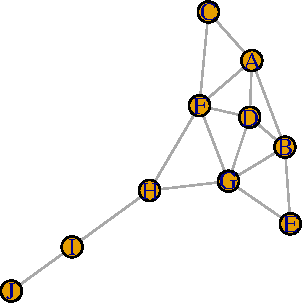
\includegraphics[width=0.25\textwidth]{FIGS/graphs-plot-union-graphs-net1-1.pdf}
$\bigcup$
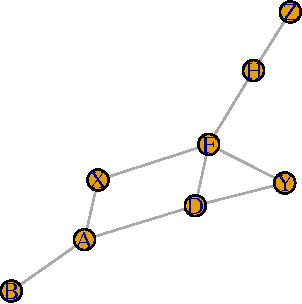
\includegraphics[width=0.25\textwidth]{FIGS/graphs-plot-union-graphs-net2-1.pdf}
$\implies$
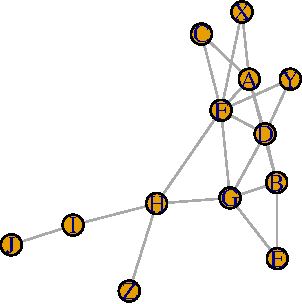
\includegraphics[width=0.3\textwidth]{FIGS/graphs-plot-union-graphs-net1Unet2-1.pdf}
\end{frame}

\begin{frame}[fragile]\frametitle{Intersection of two graphs}
\begin{knitrout}
\definecolor{shadecolor}{rgb}{0.969, 0.969, 0.969}\color{fgcolor}\begin{kframe}
\begin{alltt}
\hldef{G_inter} \hlkwb{=} \hldef{net1} \hlopt \hldef{net2}
\hlkwd{plot}\hldef{(G_inter)}
\end{alltt}
\end{kframe}
\end{knitrout}
\end{frame}

\begin{frame}
\centering
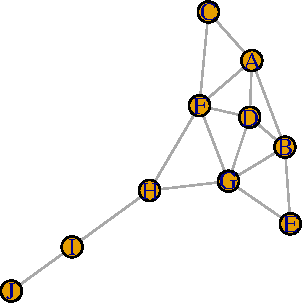
\includegraphics[width=0.25\textwidth]{FIGS/graphs-plot-union-graphs-net1-1.pdf}
$\bigcap$
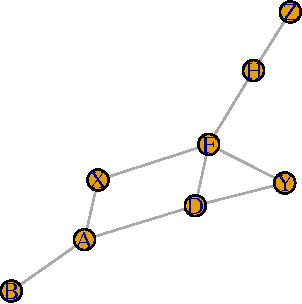
\includegraphics[width=0.25\textwidth]{FIGS/graphs-plot-union-graphs-net2-1.pdf}
$\implies$
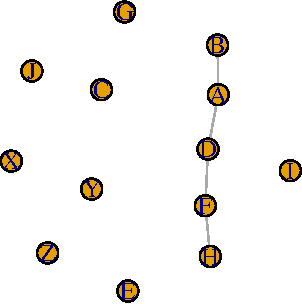
\includegraphics[width=0.3\textwidth]{FIGS/graphs-plot-intersection-graphs-net1Nnet2-1.pdf}
\end{frame}

%%%%%%%%%%%%%%%%%%%%%%
%%%%%%%%%%%%%%%%%%%%%%
\subsection{Connectedness}
\newSubSectionSlide{FIGS-transitions/Gemini_Generated_Image_fto8nofto8nofto8.jpeg}

\begin{frame}\frametitle{Connected vertices and graph, components}
\begin{definition}[{Connected vertices}]
Two vertices $u$ and $v$ in a graph $G$ are \defword{connected}\index{connected vertices} if $u=v$, or if $u\not =v$ and there exists a path in $G$ that links $u$ and $v$
\end{definition}
(For \emph{path}, see Definition~\ref{def:path} later)
\vfill
\begin{definition}[{Connected graph}]
A graph is \defword{connected}\index{connected graph} if every two vertices of $G$ are connected; otherwise, $G$ is \defword{disconnected}\index{disconnected graph}
\end{definition}
\end{frame}

\begin{frame}\frametitle{A necessary condition for connectedness}
	\begin{theorem}
		A connected graph on $p$ vertices has at least $p-1$ edges
	\end{theorem}
	\vfill
	In other words, a connected graph $G$ of order $p$ has $\text{size}(G)\geq p-1$
\end{frame}

\begin{frame}{Connectedness is an equivalence relation}
	Denote $x\equiv y$ the relation  ``$x=y$, or $x\neq y$ and there exists a path in $G$ connecting $x$ and $y$''. $\equiv$ is an equivalence relation since
	\begin{enumerate}
		\item $x\equiv y$ \hfill[reflexivity]
		\item $x\equiv y\implies y\equiv x$ \hfill[symmetry]
		\item $x\equiv y, y\equiv z\implies x\equiv z$ \hfill[transitivity]
	\end{enumerate}
	\vfill
	\begin{definition}[Connected component of a graph]
		The classes of the equivalence relation $\equiv$ partition $V$ into connected sub-graphs of $G$ called \defword{connected components} (or \defword{components} for short) of $G$
	\end{definition}
	\vfill
	A connected subgraph $H$ of a graph $G$ is a component of $G$ if $H$ is not contained in any connected subgraph of $G$ having more vertices or edges than $H$
\end{frame}



\begin{frame}{Vertex deletion \& cut vertices}
\begin{definition}[{Vertex deletion}]
If $v\in V(G)$ is a vertex of $G$, the graph $G-v$ is the graph formed from $G$ by removing $v$ and all edges incident with $v$
\end{definition}
\vfill
\begin{definition}[{Cut-vertices}]
	Let $G$ be a connected graph. Then $v$ is a \defword{cut-vertex} $G$ if $G-v$ is disconnected
\end{definition}
\end{frame}


\begin{frame}{Edge deletion \& bridges}
\begin{definition}[{Edge deletion}]
	If $e$ is an edge of $G$, the graph $G-e$ is the graph formed from $G$ by removing $e$ from $G$
\end{definition}
\vfill
\begin{definition}[{Bridge}]
An edge $e$ in a connected graph $G$ is a \defword{bridge} if $G-e$ is disconnected
\end{definition}
\vfill
\begin{theorem}
Let $G$ be a connected graph. An edge $e$ of $G$ is a bridge of $G$ $\iff$ $e$ does not lie on any cycle of $G$
\end{theorem}
(For \emph{cycle}, see Definition~\ref{def:cycle} later)
\end{frame}


%\begin{frame}\frametitle{Undirected network}
%\begin{definition}{Definition}
%A undirected network is a graph together with a function which maps the edge set into the set of real number.
%\end{definition}\end{frame}



%%%%%%%%%%%%%%%%%%%%%%
%%%%%%%%%%%%%%%%%%%%%%
\subsection{Walks, trails, paths}
\newSubSectionSlide{FIGS-transitions/Gemini_Generated_Image_fto8nofto8nofto8.jpeg}


\begin{frame}\frametitle{Walk}
\begin{definition}[{Walk}]
A \defword{walk}\index{walk, graph} in a graph $G=(V,E)$ is a non-empty alternating sequence $v_0 e_0 v_1 e_1 v_2 \dots e_{k-1} v_k$ of vertices and edges in $G$ such that $e_i=\{v_i, v_{i+1}\}$ for all $i<k$. 
This walk begins with $v_0$ and ends with $v_k$
\end{definition}
\vfill
\begin{definition}[Length of a walk]
The \defword{length} of a walk is equal to the number of edges in the walk
\end{definition}
\vfill
\begin{definition}[{Closed walk}]
If $v_0=v_k$, the walk is \defword{closed}
\end{definition}
\end{frame}


\begin{frame}\frametitle{Trail and path}
\begin{definition}[{Trail}]
If the edges in the walk are all distinct, it defines a \defword{trail} in $G=(V,E)$
\end{definition}
\vfill
\begin{definition}[{Path}]\label{def:path}
If the vertices in the walk are all distinct, it defines a \defword{path} in $G$
\end{definition}
\vfill
The sets of vertices and edges determined by a trail is a subgraph
\end{frame}


\begin{frame}\frametitle{Distance between two vertices}
\begin{definition}[{Distance between two vertices}]
The \defword{distance} $d(u,v)$ in $G=(V,E)$ between two vertices $u$ and $v$ is the length of the shortest path linking $u$ and $v$ in $G$
\vskip0.2cm
If no such path exists, we assume $d(u,v)=\infty$
\end{definition}
\end{frame}


\begin{frame}\frametitle{Circuit and cycle}
\begin{definition}[Circuit]
A trail linking $u$ to $v$, containing at least 3 edges and in which $u=v$, is a \defword{circuit}
\end{definition}
\vfill
\begin{definition}[Cycle]\label{def:cycle}
A circuit which does not repeat any vertices (except the first and the last) is a \defword{cycle} (or \defword{simple circuit})
\end{definition}
\vfill
\begin{definition}[Length of a cycle]
The \defword{length of a cycle} is its number of edges
\end{definition}
\end{frame}


\begin{frame}
\begin{definition}[{Eulerian trail}]
	A walk in an undirected multigraph $M$ that uses each edge \textbf{exactly once} is a \defword{Eulerian trail} of $M$
\end{definition}
\vfill
\begin{definition}[{Traversable graph}]
	If a graph $G$ has a Eulerian trail, then $G$ is a \defword{traversable graph}
\end{definition}
\vfill
\begin{definition}[{Eulerian circuit}]
	A circuit containing all the vertices and edges of a multigraph $M$ is a \defword{Eulerian circuit} of $M$
\end{definition}
\vfill
\begin{definition}[{Eulerian graph}]
	A graph (resp. multigraph) containing an Eulerian circuit is a \defword{Eulerian graph} (resp. \defword{Eulerian multigraph})
\end{definition}
\end{frame}

\begin{frame}{Remember Euler's bridges of K\"onigsberg?}
	Cross the 7 bridges in a single walk without recrossing any of them?
	\begin{center}
	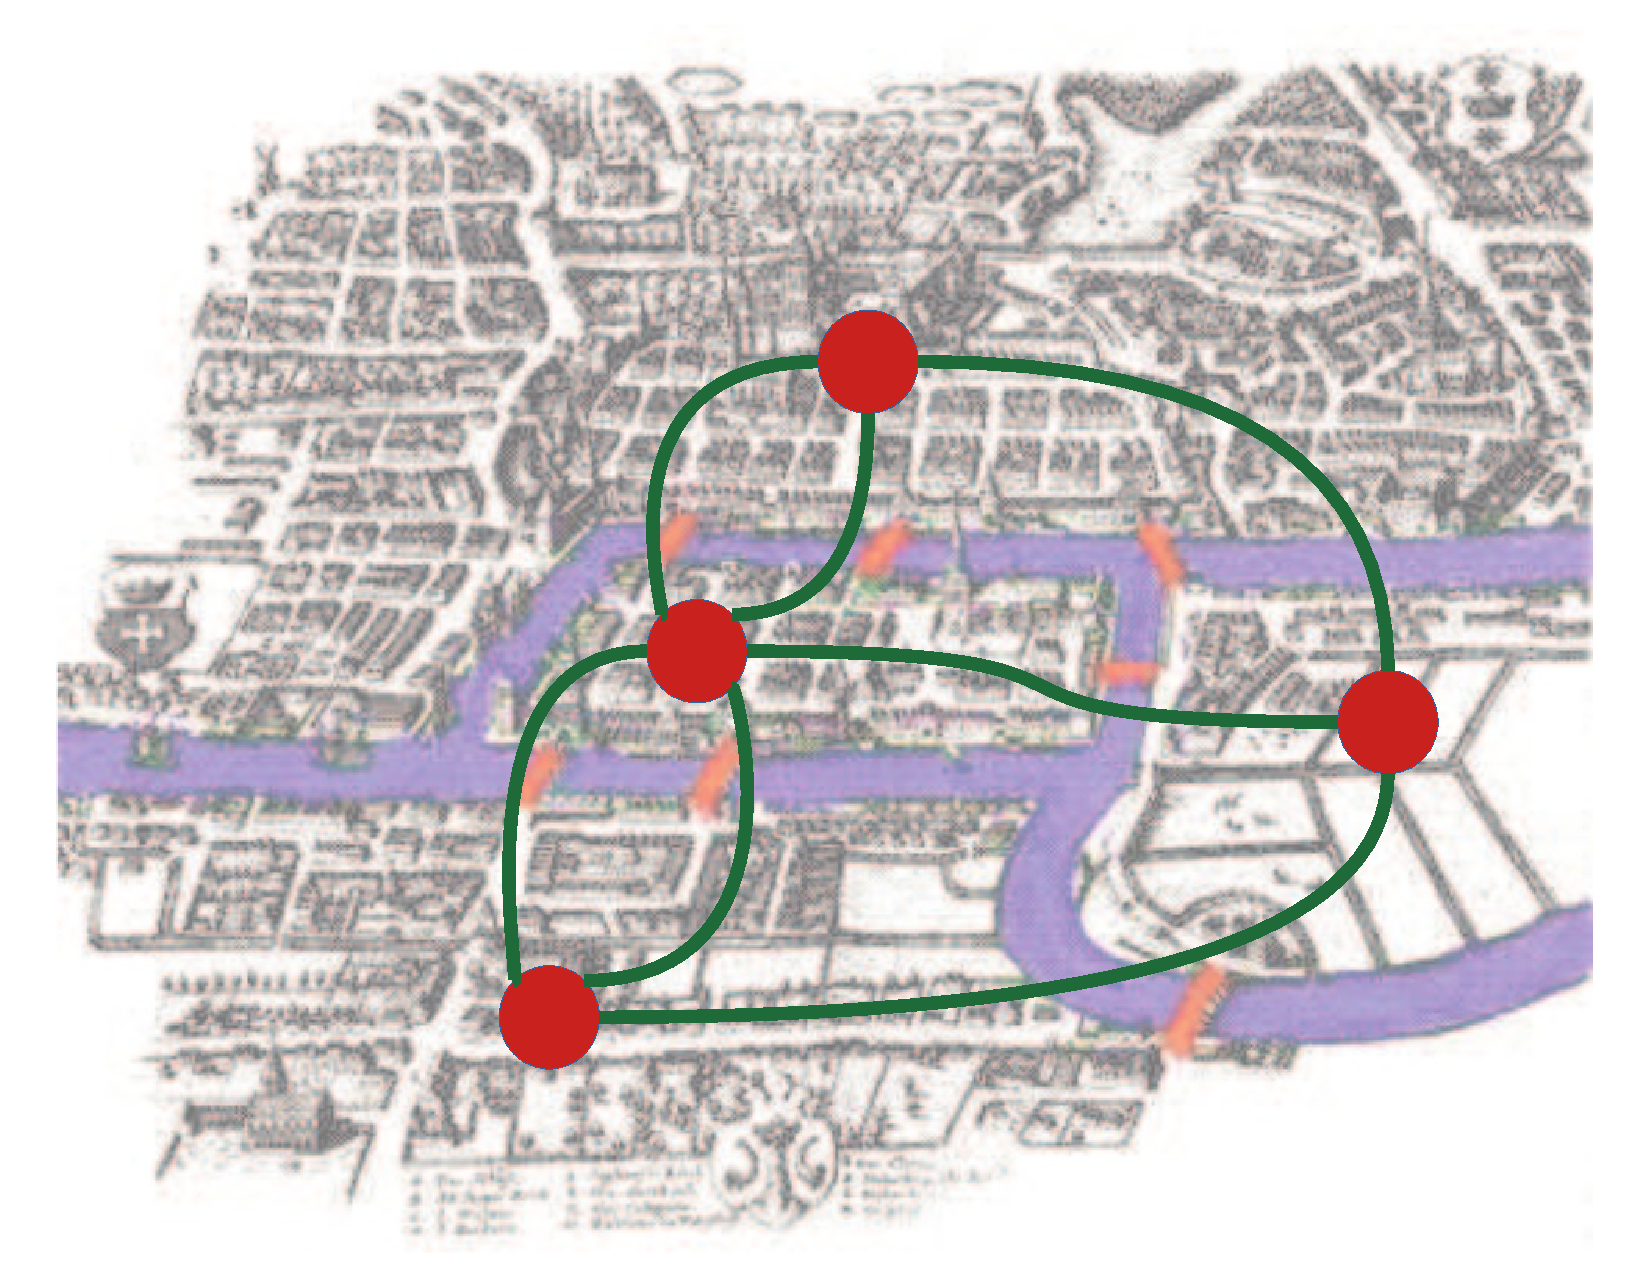
\includegraphics[width=.7\textwidth]{FIGS_slides/bridge_color_with_graph}
	\end{center}
	\begin{block}{Mathematical problem}
		Is the (multi)graph traversable? Eulerian?
	\end{block}
	\end{frame}


\begin{frame}
\begin{theorem}
	A multigraph $M$ is traversable $\iff$ $M$ is connected and has exactly two odd vertices
	\vskip0.2cm
	Furthermore, any Eulerian trail of $M$ begins at one of the odd vertices and ends at the other odd vertex
\end{theorem}
\vfill
\begin{theorem}
	A multigraph $M$ is Eulerian $\iff$ $M$ is connected and every vertex of $M$ is even
\end{theorem}
\end{frame}




\begin{frame}
	\frametitle{Fleury's algorithm to find a Eulerian \emph{trail}}
	\framesubtitle{For a connected graph with exactly 2 odd vertices}
\begin{itemize}
	\item Start at one of the odd vertices
	\item Marking your path as you move from vertex to vertex, travel along any edges you wish, but DO NOT travel along an edge that is a bridge for the graph formed by the EDGES THAT HAVE YET TO BE TRAVELED -- unless you have to
	\item Continue until every edge has been traveled
\end{itemize}
RESULT: a Eulerian trail
\end{frame}


\begin{frame}
	\frametitle{Fleury's algorithm to find a Eulerian \emph{circuit}}
	\framesubtitle{For a connected graph with no odd vertices}

	\begin{itemize}
	\item Pick any vertex as a starting point
	\item Marking your path as you move from vertex to vertex, travel along any edges you wish, but DO NOT travel along an edge that is a bridge for the graph formed by the EDGES THAT HAVE YET TO BE TRAVELED -- unless you have to
	\item Continue until you return to your starting point
\end{itemize}
RESULT: a Eulerian circuit
\end{frame}




\begin{frame}\frametitle{}
\begin{definition}[{Hamiltonian path}]
	A path containing all vertices of a graph $G$ is a \defword{Hamiltonian path} of $G$
\end{definition}
\vfill
\begin{definition}[{Traceable graph}]
	If a graph $G$ has an Hamiltonian path, then $G$ is a \defword{traceable graph}
\end{definition}
\vfill
\begin{definition}[{Hamiltonian cycle}]
	A cycle containing all vertices of a graph $G$ is a \defword{Hamiltonian cycle} of $G$
\end{definition}
\vfill
\begin{definition}[{Hamiltonian graph}]
	A graph containing a Hamiltonian cycle is a \defword{Hamiltonian graph}
\end{definition}
\end{frame}

\begin{frame}
\begin{theorem}[Dirac's theorem]
	If $G$ is a graph of order $p\geq 3$ such that $deg(v)\geq p/2$ for every vertex $v$ of $G$, then $G$ is Hamiltonian
\end{theorem}
\vfill
\begin{theorem}[Ore's theorem]
	If $G$ is a graph of order $p\geq 3$ such that for all distinct nonadjacent vertices $u$ and $v$ of $G$, $$deg(u)+deg(v)\geq p$$ 
	then $G$ is Hamiltonian
\end{theorem}
\end{frame}

%%%%%%%%%%%%%%%%%%%%%%%%%%%%%%
%%%%%%%%%%%%%%%%%%%%%%%%%%%%%%
\subsection{Complete, bipartite and other notable graphs}
\newSubSectionSlide{FIGS-transitions/Gemini_Generated_Image_fto8nofto8nofto8.jpeg}


\begin{frame}
\begin{definition}[{Complete graph}]
A graph is complete if every two of its vertices are adjacent
\end{definition}
\vfill
\begin{definition}[$n$-clique]
	A simple, complete graph on $n$ vertices is called an $n$-\defword{clique} and is often denoted $K_n$
\end{definition}
\vfill
Note that a complete graph of order $p$ is $(p-1)$-regular
\end{frame}

\begin{frame}\frametitle{Bipartite graph}
	\begin{definition}[Bipartite graph]
		A graph is \defword{bipartite} if its vertices can be partitioned into two sets $V_1$ and $V_2$, such that no two vertices in the same set are adjacent.
		This graph may be written $G=(V_1,V_2,E)$
	\end{definition}
	\vfill
	\begin{definition}[Complete bipartite graph]
		A bipartite graph in which every two vertices from the 2 different partitions are adjacent is called a \defword{complete bipartite graph}
		\vskip0.2cm
		We often denote $K_{p,q}$ a simple, complete bipartite graph with $|V_1|=p$ and $|V_2|=q$
	\end{definition}
\end{frame}

\begin{frame}\frametitle{Some specific graphs}
	\begin{definition}[{Tree}]
		Any connected graph that has no cycles is a \defword{tree}
	\end{definition}
	\begin{definition}[{Cycle $C_n$}]
		For $n\geq 3$, the \defword{cycle} $C_n$ is a connected graph of order $n$ that is a cycle on $n$ vertices
	\end{definition}
	\begin{definition}[{Path $P_n$}]
		The \defword{path} $P_n$ is a connected graph that consists of $n\geq 2$ vertices and $n-1$ edges. Two vertices of $P_n$ have degree 1 and the rest are of degree 2
	\end{definition}
	\begin{definition}[{Star $S_n$}]
		The \defword{star} of order $n$ is the complete bipartite graph $K_{1,n-1}$ (1 vertex of degree $n-1$ and $n-1$ vertices of degree 1)
	\end{definition}
\end{frame}






%%%%%%%%%%%%%%%%%%%%%%%
%%%%%%%%%%%%%%%%%%%%%%%
\subsection{Planar graphs}
\newSubSectionSlide{FIGS-transitions/Gemini_Generated_Image_fto8nofto8nofto8.jpeg}



\begin{frame}\frametitle{Planar graph}
\begin{definition}[Planar graph]
A graph is \defword{planar} if it \emph{can be} drawn in the plane with no crossing edges (except at the vertices). Otherwise, it is \defword{nonplanar}
\end{definition}
\vfill
\begin{definition}[{Plane graph}]
A \defword{plane graph} is a graph \emph{that is drawn} in the plane with no crossing edges. (This is only possible if the graph is planar)
\end{definition}
\vfill
(To see the difference, have you ever played \href{https://www.chiark.greenend.org.uk/~sgtatham/puzzles/js/untangle.html}{this game}?)
\end{frame}



\begin{frame}
Let $G$ be a plane graph
\begin{itemize}
\item the connected parts of the plane are called \defword{regions}
\item vertices and edges that are incident with a region $R$ make up a \defword{boundary} of $R$
\end{itemize}
\vfill
\begin{theorem}[{Euler's formula}]
Let $G$ be a connected plane graph with $p$ vertices, $q$ edges, and $r$ regions, then $$p-q+r=2$$
\end{theorem}
\vfill
\begin{corollary}
Let $G$ be a plane graph with $p$ vertices, $q$ edges, $r$ regions, and $k$ connected components, then $$p-q+r=k+1$$
\end{corollary}
\end{frame}


\begin{frame}
\begin{theorem}
Let $G$ be a connected planar graph with $p$ vertices and $q$ edges, where $p\geq 3$, then $$q\leq 3p-6.$$
(a maximal connected planar graph with $p$ vertices has $q=3p-6$ edges)
\end{theorem}
\vfill
\begin{corollary}
If $G$ is a planar graph, then $\delta(G)\leq 5,$
where $\delta(G)$ is the minimal degree of $G$.
(every planar graph contains a vertex of degree less than 6)
\end{corollary}
\end{frame}


\begin{frame}{Two well-known non-planar graphs}
$K_{3,3}$ and $K_5$ are nonplanar
\vfill
\begin{theorem}[{Kuratowski Theorem}]
A graph $G$ is planar $\iff$ it contains no subgraph isomorphic to $K_5$ or $K_{3,3}$ or any subdivision of $K_5$ or $K_{3,3}$
\end{theorem}
\vfill
\textbf{Note:} If a graph $G$ is nonplanar and $G$ is a subgraph of $G'$, then $G'$ is also nonplanar
\end{frame}


\subsection{Graph colouring}
\newSubSectionSlide{FIGS-transitions/Gemini_Generated_Image_fto8nofto8nofto8.jpeg}

\begin{frame}
\begin{definition}[{Colouring of a graph $G$}]
A \defword{colouring} of a graph $G$ is an assignment of colours to the vertices of $G$ such that adjacent vertices have different colours
\end{definition}
\vfill
\begin{definition}[{$n$-colouring of $G$}]
A \defword{$n$-colouring} is a colouring of $G$ using $n$ colours
\end{definition}
\vfill
\begin{definition}[{$n$-colourable}]
$G$ is \defword{$n$-colourable} if there exists a colouring of $G$ that uses $n$ colours
\end{definition}
\end{frame}


\begin{frame}
\begin{definition}[{Chromatic number}]
The \defword{chromatic number} $\chi (G)$ of a graph $G$ is the minimal value $n$ for which an $n$-colouring of $G$ exists
\end{definition}
\vfill
\begin{property}
\begin{itemize}
\item $\chi (G)=1$ $\iff$ $G$ have no edges
\item If $G=K_{n,m}$, then $\chi(G)=2$
\item If $G=K_n$, then $\chi(G)=n$
\item For any graph $G$, $$\chi (G)\leq 1+ \Delta (G)$$
where $\Delta (G)$ is the maximum degree of $G$
\item If $G$ is a planar graph, then $\chi(G) \leq 4$
\end{itemize}
\end{property}
\end{frame}


\begin{frame}\frametitle{``Real life'' problem}
What is the minimal number of colours to colour all states in the map so that two adjacent states have different colours?
\begin{center}
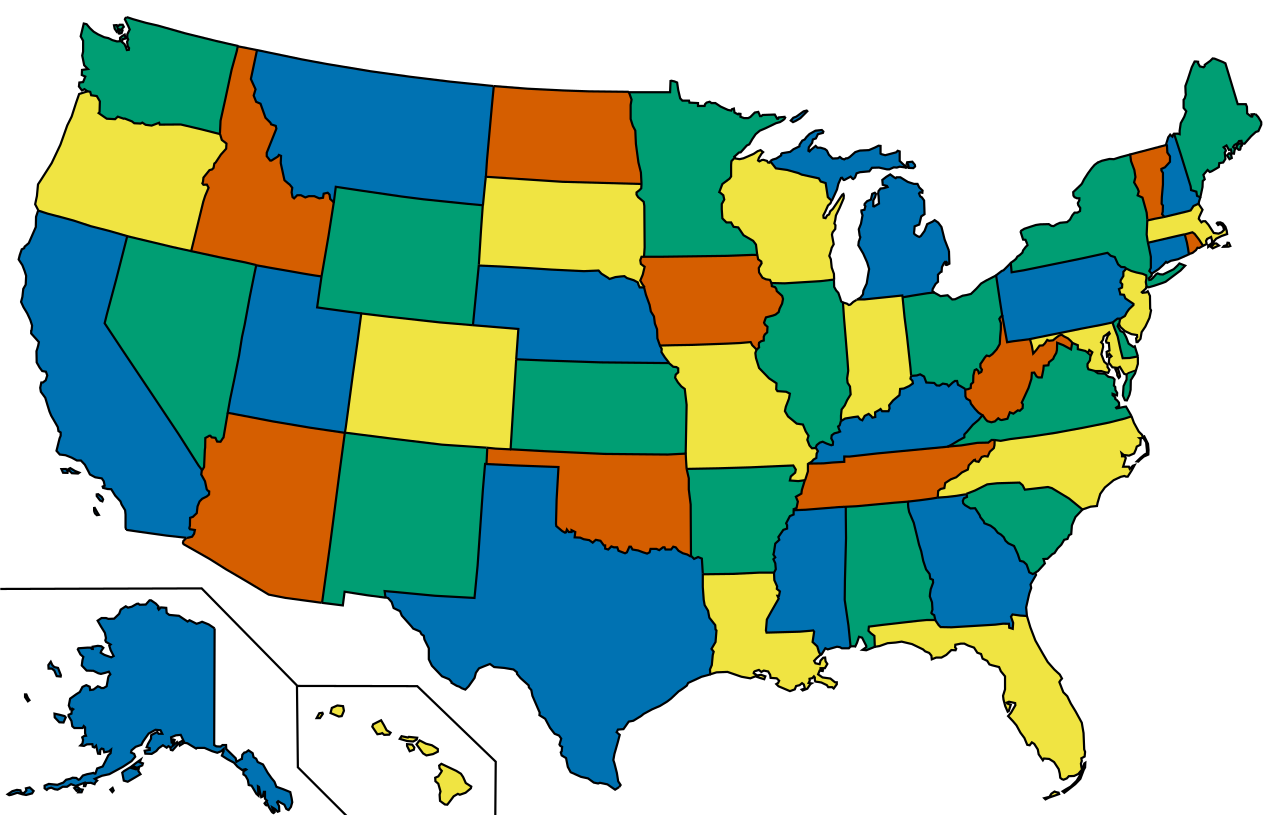
\includegraphics[width=.85\textwidth]{FIGS_slides/USA-4-colours}
\end{center}\end{frame}

\begin{frame}\frametitle{``Real life'' problem}
	What is the minimal number of colours to colour all states in the map so that two adjacent states have different colours?
	\vfill
Mathematical representation:
\begin{itemize}
\item vertices correspond to the states
\item vertices are adjacent $\iff$ the two states are adjacent (sharing an isolated point such as the ``Four Corners'' does not count)
\end{itemize}
\vfill
\begin{block}{Mathematical problem}
What is the chromatic number of the graph associated to the map?
\end{block}
\end{frame}

\begin{frame}\frametitle{Welch-Powell algorithm for colouring a graph $G$}
	\begin{enumerate}
	\item Order the vertices of $G$ by decreasing degree. (Such an ordering may not be unique since some vertices may have the same degree)
	\vfill
	\item Use one colour to paint the first vertex and to paint, in sequential order, each vertex on the list that is not adjacent to a vertex previously painted with this colour
	\vfill
	\item Start again at the top of the list and repeat the process, painting previously unpainted vertices using a second colour
	\vfill
	\item Repeat with additional colours until all vertices have been painted
\end{enumerate}\end{frame}
	
	


%%%%%%%%%%%%%%%%%%%
%%%%%%%%%%%%%%%%%%%
%%%%%%%%%%%%%%%%%%%
%%%%%%%%%%%%%%%%%%%
\section{Directed graphs}
\newSectionSlide{FIGS-transitions/Gemini_Generated_Image_fto8nofto8nofto8.jpeg}


\begin{frame} \frametitle{Definitions} 
\begin{definition}[{Digraph}]
A directed graph (or \defword{digraph}) is a pair $G=(V,A)$ of sets such that
\begin{itemize}
\item $V$ is a set of points:  $V=\{v_1,v_2,v_3,..,v_p\}$
\item $A$ is a set of ordered pairs of $V$: $A=\{(v_i,v_j),(v_i,v_k),\dots,(v_n,v_p)\}$ or $A=\{v_iv_j,v_iv_k,\dots,v_nv_p\}$
\end{itemize}
\end{definition}
\begin{definition}[{Vertex}]
The elements of $V$ are the vertices of the digraph $G$.
$V$ or $V(G)$ is the vertex set of the digraph $G$
\end{definition}
\begin{definition}[{Arc}]
The elements of $A$ are the \defword{arcs} (directed edges) of the digraph $G$.
$A$ or $A(G)$ is the arc set of the digraph $G$
\end{definition}
\end{frame}



\begin{frame}\frametitle{Digraph and binary relation}
A (simple) digraph $D$ can be defined in term of a vertex set $V$ and an irreflexive relation $R$ over $V$
\vfill
The defining relation $R$ of the digraph $G$ need not be symmetric
\end{frame}


\begin{frame}\frametitle{Directed network}
\begin{definition}[Directed network]
A directed network is a digraph together with a function $f$,
\[
f: A \rightarrow \mathbb{R},
\]
which maps the arc set $A$ into the set of real number. 
The value of the arc $uv \in A$ is $f(uv)$
\end{definition}
\end{frame}



%\begin{frame}\frametitle{Order and Size}
%\begin{definition}{Order of a graph}
%The number of vertices in $G$ is the order of $G$
%$$|V(G)|=\textrm{order of G}$$
%\end{definition}
%\begin{definition}{Size of a graph}
%The number of edges in $G$ is the size of $G$
%$$|E(G)|=\textrm{size of G}$$
%\end{definition}
%\begin{itemize}
%\item A graph having order $p$ and size $q$ is noted a $(p,q)-$graph.
%\item A graph is finite is $|V(G)|<\infty$
%\end{itemize}
%}



\begin{frame}{Loops \& Multiple arcs}
	\begin{definition}[{Loop}]
	A \defword{loop} is an arc with both the same ends; \emph{e.g.} $(u,u)$ is a loop
\end{definition}
\vfill
	\begin{definition}[{Multiple arcs}]
	\defword{Multiple arcs} (or multi-arcs) are two or more arcs connecting the same two vertices
	\end{definition}
\end{frame}
\begin{frame}{Multidigraph/Digraph}
	\begin{definition}[{Multidigraph}]
	A \defword{multidigraph} is a digraph which allows repetition of arcs or loops
	\end{definition}
	\vfill
	\begin{definition}[{Digraph}]
	In a digraph, no more than one arc can join any pair of vertices
\end{definition}
\end{frame}

\begin{frame}{Examples}
  \centering
	\def\skip{2.75cm}
	\begin{tikzpicture}[scale=0.7, 
		every node/.style={transform shape},
		auto,
		cloud/.style={minimum width={width("N-1")+2pt},
			draw, ellipse},
		connected/.style={dotted,-}]
		%% Vertices
		\node [cloud] at (0,0) (a) {$a$};
		\node [cloud] at (1*\skip,1*\skip) (b) {$b$};
		\node [cloud] at (1*\skip,-1*\skip) (c) {$c$};
		\node [cloud] at (2*\skip,0) (d) {$d$};
		%% Arcs
		\path [line, thick,bend right] (a) to node [midway, above] (TextNode) {2} (b);
		\path [line, thick] (a) to node [midway, above] (TextNode) {3} (b);
		\path [line, thick,bend left] (a) to node [midway, above] (TextNode) {4} (b);
		\path [line, thick, looseness=5] (b) to node [midway, above] (TextNode) {5} (b);
		\path [line, thick, looseness=15] (b) to node [midway, above] (TextNode) {6} (b);
		\path [line, thick] (c) to node [midway, left] (TextNode) {7} (b);
		\path [line, thick] (c) to node [midway, above] (TextNode) {1} (a);
		\path [line, thick, bend left] (d) to node [midway, above] (TextNode) {8} (c);
		\path [line, thick, bend right] (d) to node [midway, above] (TextNode) {9} (c);
		\path [line, thick, looseness=5] (d) to node [midway, above] (TextNode) {10} (d);
	\end{tikzpicture}
	\begin{tikzpicture}[scale=0.7, 
		every node/.style={transform shape},
		auto,
		cloud/.style={minimum width={width("N-1")+2pt},
			draw, ellipse},
		connected/.style={dotted,-}]
		%% Vertices
		\node [cloud] at (0,0) (x1) {$x_1$};
		\node [cloud] at (1*\skip,1*\skip) (x2) {$x_2$};
		\node [cloud] at (2*\skip,1*\skip) (x3) {$x_3$};
		\node [cloud] at (1.5*\skip,0) (x4) {$x_4$};
		\node [cloud] at (2.5*\skip,0*\skip) (x5) {$x_5$};
		\node [cloud] at (2.5*\skip,1*\skip) (x6) {$x_6$};
		%% Arcs
		\path [line, thick,bend left] (x1) to node [midway, above] (TextNode) {1} (x2);
		\path [line, thick,bend left] (x2) to node [midway, below] (TextNode) {2} (x1);
		\path [line, thick, looseness=5] (x2) to node [midway, above] (TextNode) {3} (x2);
		\path [line, thick] (x2) to node [midway, above] (TextNode) {4} (x3);
		\path [line, thick] (x2) to node [midway, below] (TextNode) {5} (x4);
		\path [line, thick] (x4) to node [midway, below] (TextNode) {6} (x3);
		\path [line, thick, looseness=5, below] (x6) to node [midway, above] (TextNode) {7} (x6);
		\path [line, thick] (x6) to node [midway, right] (TextNode) {8} (x5);
	\end{tikzpicture}
\end{frame}

\begin{frame}
	Let $G=(V,A)$ be a digraph
	\begin{definition}[Arc endpoints]
	For an arc $u=(x,y)$, vertex $x$ is the \defword{initial endpoint}, and vertex $y$ is the \defword{terminal endpoint}
	\end{definition}
	\begin{definition}[{Predecessor - Successor}]
		If $(u,v)\in A(G)$ is an arc of $G$, then
		\begin{itemize}
			\item  $u$ is a \defword{predecessor} of $v$
			\item  $v$ is a \defword{successor} of $u$
		\end{itemize}
	\end{definition}
	\begin{definition}[Neighbours of a vertex]
	Let $x\in V$ be a vertex. The \defword{neighbours} of $x$ is the set $\Gamma(x) = \Gamma^+_G(x)\cup\Gamma^-_G(x)$, where $\Gamma^+_G(x)$ and $\Gamma^-_G(x)$ are, respectively, the set of successors and predecessors of $v$
	\end{definition}
\end{frame}
	
	
\begin{frame}{Sources and sinks}
	\begin{definition}[{Directed away - Directed towards}]
		If $a=(u,v)\in A(G)$ is an arc of $G$, then
		\begin{itemize}
			\item the arc $a$ is said to be \defword{directed away} from $u$
			\item the arc $a$ is said to be \defword{directed towards} $v$
		\end{itemize}
	\end{definition}
	\vfill
	\begin{definition}[{Source - Sink}]
		\begin{itemize}
			\item Any vertex which has no arcs directed towards it is a \defword{source}
			\item Any vertex which has no arcs directed away from it is a \defword{sink}
		\end{itemize}
	\end{definition}
\end{frame}

\begin{frame}{Adjacent arcs}
	\begin{definition}[Adjacent arcs]
		Two arcs are \defword{adjacent} if they have at least one endpoint in common
	\end{definition}
\end{frame}

\begin{frame}{Arcs incident to a subset of arcs}
	\begin{definition}[Arc incident out of $X\subset A(G)$]
		If the initial endpoint of an arc $u$ belongs to $X\subset A(G)$ and if the terminal endpoint of arc $u$ does not belong to $X$, then $u$ is said to be \defword{incident out of} $X$; we write $u\in\omega^+(X)$
		\vskip0.2cm
		Similarly, we define an \defword{arc incident into} $X$ and the set $\omega^-(X)$
		\vskip0.2cm
		Finally, the set of arcs \defword{incident to} $X$ is denoted
		\[
		\omega(X) = \omega^+(X)\cup\omega^-(X)
		\]
	\end{definition}
\end{frame}

\begin{frame}
	\begin{definition}[Subgraph of $G$ generated by $A\subset V$]
		The \defword{subgraph} of $G$ generated by $A$ is the graph with $A$ as its vertex set and with all the arcs in $G$ that have both their endpoints in $A$. If $G=(V,\Gamma)$ is a 1-graph, then the subgraph generated by $A$ is the 1-graph $G_A=(A,\Gamma_A)$ where
		\[
		\Gamma_A(x)=\Gamma(x)\cap A\qquad (x\in A)
		\]
	\end{definition}
	\vfill
	\begin{definition}[Partial graph of $G$ generated by $V\subset U$]
		\label{def:partial_graph}
		The graph $(X,V)$ whose vertex set is $X$ and whose arc set is $V$. 
		In other words, it is graph $G$ without the arcs $U-V$
	\end{definition}
	\vfill
	\begin{definition}[Partial subgraph of $G$]
		A partial subgraph of $G$ is the subgraph of a partial graph of $G$
	\end{definition}
\end{frame}



%%%%%%%%%%%%%%%%%%%%%%%%%%
%%%%%%%%%%%%%%%%%%%%%%%%%%
\subsection{Degrees in digraphs}
\newSubSectionSlide{FIGS-transitions/Gemini_Generated_Image_fto8nofto8nofto8.jpeg}

\begin{frame}{Degree}
	Let $v$ be a vertex of a digraph $G=(V,A)$
	\begin{definition}[{Outdegree of a vertex}]
	The number of arcs directed away from a vertex $v$, in a digraph is called the \defword{outdegree} of $v$ and is written $d^+_G(v)$
	\end{definition}
	\begin{definition}[{Indegree of a vertex}]
	The number of arcs directed towards a vertex $v$, in a digraph is called the \defword{indegree} of $v$ and is written $d^-_G(v)$
	\end{definition}
	\begin{definition}[{Degree}]
	For any vertex $v$ in a digraph, the \defword{degree}\index{degree, digraph} of $v$ is defined as 
	\[
		d_G(v)=d^+_G(v)+d^-_G(v)
	\]
	\end{definition}
\end{frame}



\begin{frame}
	\begin{theorem}
		For any (di)graph, the sum of the degrees of the vertices equals twice the number of edges (arcs)
	\end{theorem}
	\begin{corollary}
		In any (di)graph, the sum of the degrees of the vertices is a nonnegative even integer
	\end{corollary}
	\begin{theorem}
		If $G$ is a digraph with vertex set $V(G)=\{v_1, \dots , v_p\}$ and $q$ arcs, then $$\sum_{i=1}^p d^+_G(v_i)=\sum_{i=1}^p d^-_G(v_i)=q$$
	\end{theorem}
\end{frame}

\begin{frame}
	\begin{definition}[{Regular digraph}]
		A digraph $G$ is $r$-regular if $d_G^+(v)=d_G^-(v)=r$ for all $v\in V(G)$
\end{definition}\end{frame}

\begin{frame}{Symmetric/antisymmetric digraphs}
	\begin{definition}[Symmetric digraph]
		Let $G=(V,A)$ be a digraph with associated binary relation $R$.
		If $R$ is \emph{symmetric}, the digraph is symmetric
	\end{definition}
	\vfill
	\begin{definition}[Anti-symmetric digraph]
		Let $G=(V,A)$ be a digraph with associated binary relation $R$.
		The digraph $G$ is \defword{anti-symmetric} if
		\[
		xRy \implies y\cancel R x
		\]
	\end{definition}
	\vfill
	\begin{definition}[Symmetric multidigraph]
		Let $G=(V,A)$ be a multidigraph. $G$ is symmetric if $\forall x,y\in V(G)$, the number of arcs from $x$ to $y$ equals the number of arcs from $y$ to $x$
	\end{definition}
\end{frame}


%%%%%%%%%%%%%%%%%%%
%%%%%%%%%%%%%%%%%%%
\subsection{Walks, paths, etc.}
\newSubSectionSlide{FIGS-transitions/Gemini_Generated_Image_fto8nofto8nofto8.jpeg}

\begin{frame}\frametitle{Walks}
	Let $G=(V,A)$ be a digraph.
	\begin{definition}[Directed walk]
	A \defword{directed walk} in a digraph $G$ is a non-empty alternating sequence $v_0 a_0 v_1 a_1 v_2 \dots a_{k-1} v_k$ of vertices and arcs in $G$ such that $a_i=(v_i, v_{i+1})$ for all $i<k$. 
	This walk begins with $v_0$ and ends with $v_k$
	\end{definition}
	\begin{definition}[{Length of a directed walk}]
	The length of a directed walk is equal to the number of arcs in the directed walk
	\end{definition}
	\begin{definition}[{Closed walk}]
	If $v_0=v_k$, the walk is closed
	\end{definition}
\end{frame}


\begin{frame}\frametitle{Trails}
	Let $G=(V,A)$ be a digraph.
	\begin{definition}[{Directed trail}]
	A directed walk in $G$ in which all arcs are distinct is a \defword{directed trail} in $G$
	\end{definition}
	\begin{definition}[Directed path]
	A directed walk in $G$ in which all vertices are distinct is a \defword{directed path} in $G$
	\end{definition}
	\begin{definition}[{Directed cycle}]
	A closed walk is a \defword{directed cycle} if it contains at least three vertices and all its vertices are distinct except for $v_0=v_k$
	\end{definition}
\end{frame}

\begin{frame}{Examples of directed cycles}
	\begin{minipage}{0.5\textwidth}
		\centering
		\def\skip{2.75cm}
		\begin{tikzpicture}[scale=1, 
			every node/.style={transform shape},
			auto,
			cloud/.style={minimum width={width("N-1")+2pt},
				draw, ellipse},
			connected/.style={dotted,-}]
			%% Vertices
			\node [cloud] at (0,0) (a) {$a$};
			\node [cloud] at (1*\skip,0) (b) {$b$};
			\node [cloud] at (0.5*\skip,1*\skip) (c) {$c$};
			\node [cloud] at (1.5*\skip,1*\skip) (d) {$d$};
			%% Arcs
			\path [line, thick] (a) to node [midway, above] (TextNode) {1} (b);
			\path [line, thick, bend left] (a) to node [midway, above] (TextNode) {2} (c);
			\path [line, thick] (b) to node [midway, above] (TextNode) {6} (c);
			\path [line, thick] (b) to node [midway, above] (TextNode) {4} (d);
			\path [line, thick, bend left] (c) to node [midway, above] (TextNode) {3} (a);
			\path [line, thick] (c) to node [midway, above] (TextNode) {5} (d);
		\end{tikzpicture}
	\end{minipage}
	\begin{minipage}{0.48\textwidth}
		Cycles:
		\begin{itemize}
			\item $\bmu^1=(1,6,2)=[abca]$
			\item $\bmu^2=(1,6,3)=[abca]$
			\item $\bmu^3=(2,3)=[aca]$
			\item $\bmu^4=(1,4,5,2)=[abdca]$
			\item $\bmu^5=(6,5,4)=[acdb]$
			\item $\bmu^6=(1,4,5,3)=[abdca]$
		\end{itemize}
	\end{minipage}
\end{frame}


%%%%%%%%%%%%%%%%%%%%%%%%%%
%%%%%%%%%%%%%%%%%%%%%%%%%%
\subsection{Connectivity in digraphs}
\newSubSectionSlide{FIGS-transitions/Gemini_Generated_Image_fto8nofto8nofto8.jpeg}

\begin{frame}\frametitle{Definitions}
	%Let $D=(V,A)$ be a digraph.
	\begin{definition}[{Underlying graph}]
	Given a digraph, the undirected graph with each arc replaced by an edge is called the \defword{underlying graph}
	\end{definition}
	\vfill
	\begin{definition}[{Weakly connected digraph}]
	If the underlying graph is a connected graph, then the digraph is \defword{weakly connected}
	\end{definition}
	\vfill
	\begin{definition}[{Strongly connected digraph}]
	A digraph $G$ is \defword{strongly connected} if for every two distinct vertices $u$ and $v$ of $G$, there exists a directed path from $u$ to $v$
	\end{definition}
	\vfill
	\begin{definition}[{Disconnected digraph}]
	A digraph is said to be \defword{disconnected}\index{disconnected digraph} if it is not weakly connected
	\end{definition}
\end{frame}

\begin{frame}{Strong connectedness is an equivalence relation}
Denote $x\equiv y$ the relation  ``$x=y$, or $x\neq y$ and there exists a directed path in $G$ from $x$ to $y$''. $\equiv$ is an equivalence relation since
\begin{enumerate}
	\item $x\equiv y$ \hfill[reflexivity]
	\item $x\equiv y\implies y\equiv x$ \hfill[symmetry]
	\item $x\equiv y, y\equiv z\implies x\equiv z$ \hfill[transitivity]
\end{enumerate}
\begin{definition}[Connected component of a graph]
	\label{def:strong_components}
	Sets of the form 
	\[
	A(x_0)=\{x:x\in V, x\equiv x_0\}	
	\]
	are equivalence classes. 
	They partition $V$ into strongly connected sub-digraphs of $G$ called \defword{strongly connected components} (or \defword{strong components}) of $G$
\end{definition}
A strong component in $G$ is a maximal strongly connected subdigraph of $G$
\end{frame}


\begin{frame}
	\begin{theorem}[Properties]
		Let $G=(V,A)$ be a digraph
	\begin{itemize}
	\item If $G$ is strongly connected, it has only one strongly connected component
	\item The strongly connected components partition the vertices $V(G)$, with every vertex in exactly one strongly connected component
	\end{itemize}
	\end{theorem}
\end{frame}



\begin{frame}\frametitle{Algorithm for determining strongly connected components in $G=(V,A)$}
	\begin{itemize}
	\item Determine the strongly connected component $C(v)$ containing the vertex $v$; if $V-C(v)$ is non-empty, re-do the same operation on the sub-digraph $G'=(V-C(v),A')$
	\item To determine $C(v)$, the strongly connected component containing $v$: let $v$ be a vertex of a digraph , which is not already in any strongly connected component
	%Set $C(v)=\{v\}$ the strongly connected component containing $v$.
	%
	%
	%
	%
	%%Repeat until $V-C(v)=\emptyset$:
	%Do for any $v\in V-C(v)$
	\begin{enumerate}
	\item Mark the vertex $v$ with $\pm$
	\item Mark with $+$ all successors (not already marked with $+$) of a vertex marked with $+$
	\item Mark with $-$ all predecessors (not already marked with $-$) of a vertex marked with $-$
	\item Repeat until no more possible marking with $+$ or $-$
	\end{enumerate}
	All vertices marked with $\pm$ belong to the same strongly connected component $C(v)$ containing the vertex $v$
	\end{itemize}
\end{frame}

\begin{frame}\frametitle{Condensation of a digraph}
	\begin{definition}[{Condensation of a digraph}]
		The condensation $G^*$ of a digraph $G$ is a digraph having as vertices the strongly connected components (SCC) of $G$ and such that there exists an arc in $G^*$ from a SCC $C_i$ to another SCC $C_j$ if there is an arc in $G$ from some vertex of $S_i$ to a vertex of $S_j$
	\end{definition}
\end{frame}


\begin{frame} 
	\begin{definition}[Articulation set]
		For a connected graph, a set $X$ of vertices is called an \defword{articulation set} (or a \defword{cutset}) if the subgraph of $G$ generated by $V-X$ is not connected
	\end{definition}
	\vfill
	\begin{definition}[Stable set]
		A set $S$ of vertices is called a \defword{stable set} if no arc joins two distinct vertices in $S$
	\end{definition}
	\vfill
\end{frame}




%%%%%%%%%%%%%%%%%
%%%%%%%%%%%%%%%%%
\subsection{Orientable graphs}
\newSubSectionSlide{FIGS-transitions/Gemini_Generated_Image_fto8nofto8nofto8.jpeg}

\begin{frame}\frametitle{Orientation}
\begin{definition}[Orienting a graph]
Given a connected \emph{graph}, we describe the act of assigning a direction to each edge (edge $\rightarrow$ arc) as \defword{orienting the graph}
\end{definition}
\vfill
\begin{definition}[{Strong orientation}]
If the digraph resulting from orienting a graph is strongly connected, the orientation is a \defword{strong orientation}
\end{definition}
\end{frame}
 
 
\begin{frame}\frametitle{Orientable graph}
\begin{definition}[Orientable graph]
A connected graph $G$ is \defword{orientable} if it admits a strong orientation
\end{definition}
\vfill
\begin{theorem}
A connected graph $G=(V,E)$ is orientable $\iff$ $G$ contains no bridges
\end{theorem}
(in other words, iff every edge is contained in a cycle)
\end{frame}
 






%%%%%%%%%%%%%%%%%%%%%%%%%%
%%%%%%%%%%%%%%%%%%%%%%%%%%
%%%%%%%%%%%%%%%%%%%%%%%%%%
%%%%%%%%%%%%%%%%%%%%%%%%%%
\section{Matrices associated to a graph/digraph}

\begin{frame}{Matrices associated to a graph/digraph}
	There are multiple matrices associated to a graph/digraph
	\vfill
	The branch of graph theory that studies the properties of matrices derived from graphs and uses of these matrices in determining graph properties is \emph{spectral graph theory}
	\vfill
	Graphs greatly simplify some problems in linear algebra and vice versa
\end{frame}

\subsection{Adjacency matrices}
\newSubSectionSlide{FIGS-transitions/Gemini_Generated_Image_fto8nofto8nofto8.jpeg}


\begin{frame}\frametitle{Adjacency matrix (undirected case)}
	Let $G=(V,E)$ be a graph of order $p$ and size $q$, with vertices $v_1, \ldots, v_p$ and edges $e_1, \dots , e_q$
	\begin{definition}[{Adjacency matrix}]
		The \defword{adjacency matrix} is $$M_A=M_A(G)=[m_{ij}]$$ is a $p\times p$ matrix in which
		$$m_{ij}=\left \{ 
		\begin{array}{cc}
			1 & \textrm{if } v_i \textrm{ and } v_j \textrm{ are adjacent}\\
			0 & \textrm{otherwise}
		\end{array}
		\right .
		$$
	\end{definition}
\end{frame}

\begin{frame}
	\begin{theorem}[{Adjacency matrix and degree}]
		The sum of the entries in row $i$ of the adjacency matrix is the degree of $v_i$ in the graph
	\end{theorem}
	\vfill
	We often write $A(G)$ and, reciprocally, if $A$ is an adjacency matrix, $G(A)$ the corresponding graph
	\vfill
	$G$ undirected $\implies$ $A(G)$ symmetric
	\vfill
	$A(G)$ has nonzero diagonal entries if $G$ is not simple
\end{frame}

\begin{frame}\frametitle{Adjacency matrix (directed case)}
	Let $G=(V,A)$ be a digraph of order $p$ with vertices $v_1,\ldots,v_p$
	\begin{definition}[Adjacency matrix]
	The \defword{adjacency matrix} $M=M(G)=[m_{ij}]$ is a $p\times p$ matrix in which
	$$m_{ij}=\left \{ 
	\begin{array}{cl}
	1 & \textrm{if arc } v_iv_j \in A\\
	0 & \textrm{otherwise}
	\end{array}
	\right .
	$$
	\end{definition}
\end{frame}

\begin{frame}
	\begin{theorem}[{Properties}]
	\begin{itemize}
	\item $M$ is not necessarily symmetric
	\item The sum of any column of $M$ is equal to the number of arcs directed towards $v_j$
	\item The sum of the entries in row $i$ is equal to the number of arcs directed away from vertex $v_i$
	\item The $(i,j)-$entry of $M^n$ is equal to the number of walks of length $n$ from vertex $v_i$ to $v_j$
	\end{itemize}
	\end{theorem}
\end{frame}
	
\begin{frame}
	\begin{definition}[Multiplicity of a pair]
		The \defword{multiplicity} of a pair $x,y$ is the number $m_G^+(x,y)$ of arcs with initial endpoint $x$ and terminal endpoint $y$. Let
		\begin{align*}
			m_G^-(x,y) &= m_G^+(y,x) \\
			m_G(x,y) &= m_G^+(x,y)+m_G^-(x,y)
		\end{align*}
		If $x\neq y$, then $m_G(x,y)$ is number of arcs with both $x$ and $y$ as endpoints. If $x=y$, then $m_G(x,y)$ equals twice the number of loops attached to vertex $x$. If $A,B\subset V$, $A\neq B$, let
		\begin{align*}
			m_G^+(A,B) &= \{u:u\in U, u=(x,y),x\in A,y\in B\} \\
			m_G(A,B) &= m_G^+(A,B)+m_G^+(A,B)
		\end{align*}
	\end{definition}
\end{frame}

\begin{frame}{Adjacency matrix of a multigraph}
\begin{definition}[Matrix associated with $G$]
	If $G$ has vertices $x_1,x_2,\ldots,x_n$, then the \defword{matrix associated} with $G$ is 
	\[
	a_{ij}=m_G^+(x_i,x_j)
	\]
\end{definition}
\vfill
\begin{definition}[Adjacency matrix]
	The matrix $a_{ij}+a_{ji}$ is the \defword{adjacency matrix} associated with $G$
\end{definition}
\end{frame}

\begin{frame}{Adjacency matrix (multigraph case)}
	\begin{definition}[Adjacency matrix of a multigraph]
		$G$ an $\ell$-graph, then the adjacency matrix $M_A=[m_{ij}]$ is defined as follows
		\[
		m_{ij} = \begin{cases}
			k & \text{if arc there are $k$ arcs } (i,j)\in U\\
			0 & \text{otherwise}
		\end{cases}
		\]
		with $k\leq \ell$
	\end{definition}
	\vfill
	$G$ undirected $\implies$ $M_A(G)$ symmetric
	\vfill
	$M_A(G)$ has nonzero diagonal entries if $G$ is not simple.
\end{frame}

\begin{frame}{Weighted adjacency matrices}
	Sometimes, adjacency matrices (typically for 1-graphs) have real entries, usually positive
	\vfill
	This means that the arcs/edges have been given a weight
\end{frame}


\begin{frame}
	\begin{theorem}[{Number of walks of length $n$}]
		Let $A$ be the adjacency matrix of a graph $G=(V(G),E(G))$, where $V(G)=\{v_1,v_2, \dots , v_p\}$. Then the $(i,j)-$entry of $A^n$, $n\geq 1$, is the number of different walks linking $v_i$ to $v_j$ of length $n$ in $G$.
	\end{theorem}
	(two walks of the same length are equal if their edges occur in exactly the same order)
	
	Example: let $A$ be the adjacency matrix of a graph $G=(V(G),E(G))$. 
	\begin{itemize}
		\item the $(i,i)-$entry of $A^2$ is equal to the degree of $v_i$.
		\item the $(i,i)-$entry of $A^3$ is equal to twice the number of $C_3$ containing $v_i$.
	\end{itemize}
\end{frame}


%%%%%%%%%%%%%%%%%%%%%%%%%%%%%
%%%%%%%%%%%%%%%%%%%%%%%%%%%%%
\subsection{Other matrices associated to a graph/digraph}
\newSubSectionSlide{FIGS-transitions/Gemini_Generated_Image_fto8nofto8nofto8.jpeg}

\begin{frame}\frametitle{Incidence matrix (undirected case)}
	Let $G=(V,E)$ be a graph of order $p$, and size $q$, with vertices $v_1, \ldots , v_p$, and edges $e_1, \ldots , e_q$
	\begin{definition}[{Incidence matrix}]
		The incidence matrix is $$B=B(G)=[b_{ij}]$$ is that $p\times q$ matrix in which
		$$b_{ij}=\left \{ 
		\begin{array}{cc}
			1 & \textrm{if } v_i \textrm{ is incident with } e_j\\
			0 & \textrm{otherwise}
		\end{array}
		\right .
		$$
	\end{definition}
	\begin{theorem}[{Incidence matrix and degrees}]
		The sum of the entries in row $i$ of the incidence matrix is the degree of $v_i$ in the graph
	\end{theorem}
\end{frame}


\begin{frame}\frametitle{Incidence matrix (directed case)}
	Let $G=(V,A)$ be a digraph of order $p$ and size $q$, with vertices $v_1, \ldots , v_p$ and arcs $a_1, \ldots , a_q$
	\begin{definition}[Incidence matrix]
	The \defword{incidence matrix} $B=B(G)=[b_{ij}]$ is a $p\times q$ matrix in which
	$$b_{ij}=\left \{ 
	\begin{array}{cl}
	1 & \textrm{if arc } a_j  \textrm{ is directed away from a vertex } v_i\\
	-1 & \textrm{if arc } a_j  \textrm{ is directed towards a vertex } v_i\\
	0 & \textrm{otherwise}
	\end{array}
	\right .
	$$
	\end{definition}
\end{frame}
	



\begin{frame}{Spectrum of a graph}
	We will come back to this later, but for now..
	\vfill
	\begin{definition}[Spectrum of a graph]
		The \defword{spectrum} of a graph $G$ is the spectrum (set of eigenvalues) of its associated adjacency matrix $M(G)$
	\end{definition}
	\vfill
	This is regardless of the type of adjacency matrix or graph
\end{frame}





\begin{frame}{Degree matrix}
	\begin{definition}[Degree matrix]
		The \defword{degree} matrix $D=[d_{ij}]$ for $G$ is a $n \times n$ diagonal matrix defined as
		\[
			d_{ij} = \begin{cases}
				d_G(v_i) & \text{if } i = j \\
				0 & \text{otherwise}
			\end{cases}
		\]
	\end{definition}
\vfill
In an undirected graph, this means that each loop increases the degree of a vertex by two
\vfill
In a directed graph, the term ``degree'' may refer either to indegree (the number of incoming edges at each vertex) or outdegree (the number of outgoing edges at each vertex)
\end{frame}

\begin{frame}{Laplacian matrix}
\begin{definition}[Laplacian matrix]
	$G=(V,A)$ a simple graph with $n$ vertices. The \defword{Laplacian} matrix is 
	\[
		L=D(G)-M(G)
	\]
	where $D(G)$ is the degree matrix and $M(G)$ is the adjacency matrix
\end{definition}
\end{frame}

\begin{frame}{Laplacian matrix (continued)}
$G$ simple graph $\implies$ $M(G)$ only contains 1 or 0 and its diagonal elements are all 0
\vfill
For directed graphs, either the indegree or outdegree is used, depending on the application
\vfill
Elements of $L$ are given by
\[
\ell_{ij}=\begin{cases}
	d_G(v_{i}) & \text{if } i=j\\
	-1 & \text{if } i\neq j \text{ and } v_{i} 
	\text{ is adjacent to }v_{j}\\
	0 & \text{otherwise}
\end{cases}
\]
\end{frame}


\begin{frame}\frametitle{Distance matrix}
	Let $G$ be a graph of order $p$ with vertices $v_1, \ldots , v_p$
	\begin{definition}[Distance matrix]
	The distance matrix $\Delta(G)=[d_{ij}]$ is a $p\times p$ matrix in which
	$$\delta_{ij}=
	d_G(v_i,v_j)
	$$
	Note $\delta_{ii}=0$ for $i=1,\ldots, p$
	\end{definition}
\end{frame}

\begin{frame}
	\begin{property}
		\begin{itemize}
		\item $M$ is not necessarily symmetric
		\item The sum of any column of $M$ is equal to the number of arcs directed towards $v_j$
		\item The sum of the entries in row $i$ is equal to the number of arcs directed away from vertex $v_i$
		\item The $(i,j)-$entry of $M^n$ is equal to the number of walks of length $n$ from vertex $v_i$ to $v_j$
		\end{itemize}
	\end{property}
\end{frame}



\subsection{Linking graphs and linear algebra}
\newSubSectionSlide{FIGS-transitions/Gemini_Generated_Image_fto8nofto8nofto8.jpeg}

\begin{frame}{Counting paths}
	\begin{theorem}
		$G$ a digraph and $M_A(G)$ its adjacency matrix. Denote $P=[p_{ij}]$ the matrix $P=M_A^k$. Then $p_{ij}$ is the number of distinct paths of length $k$ from $i$ to $j$ in $G$
	\end{theorem}
	\vfill
	\begin{definition}[Irreducible matrix]
		A matrix $A\in\M_n$ is \defword{reducible} if $\exists P\in\M_n$, permutation matrix, s.t. $P^TAP$ can be written in block triangular form. If no such $P$ exists, $A$ is \defword{irreducible}
	\end{definition}
	\vfill
	\begin{theorem}
		$A$ irreducible $\iff$ $G(A)$ strongly connected
	\end{theorem}
\end{frame}

\begin{frame}
	\begin{theorem}
		Let $A$ be the adjacency matrix of a graph $G$ on $p$ vertices. 
		A graph $G$ on $p$ vertices is connected $\iff$ $$I+A+A^2+\dots+A^{p-1}=C$$
		has no zero entries
	\end{theorem}
	\vfill
	\begin{theorem}
		Let $M$ be the adjacency matrix of a digraph $D$ on $p$ vertices. 
		A digraph $D$ on $p$ vertices is strongly connected $\iff$ $$I+M+M^2+\dots+M^{p-1}=C$$
		has no zero entries
	\end{theorem}
\end{frame}


\begin{frame}{Nonnegative matrix}
\vfill
$A=[a_{ij}]\in\M_n(\IR)$ \defword{nonnegative} if $a_{ij}\geq 0$ $\forall i,j=1,\ldots,n$; $\bv\in\IR^n$ nonnegative if $v_i\geq 0$ $\forall i=1,\ldots,n$.  \defword{Spectral radius} of $A$
\[
\rho(A) = \max_{\lambda\in\mathsf{Sp}(A)}\{|\lambda|\}
\]
$\mathsf{Sp}(A)$ the \defword{spectrum} of $A$
\end{frame}

\begin{frame}{Perron-Frobenius (PF) theorem}
\begin{theorem}[PF -- Nonnegative case]
$0\leq A\in\M_n(\IR)$. Then $\exists\bv\geq\b0$ s.t. 
\[
	A\bv=\rho(A)\bv
\]
\end{theorem}
\vfill
\begin{theorem}[PF -- Irreducible case]
	\label{th:PF}
	Let $0\leq A\in \M_n(\IR)$ irreducible. Then $\exists\bv>\b0$ s.t.
	\[
		A\bv=\rho(A)\bv
	\]
	$\rho(A)>0$ and with algebraic multiplicity 1.
	No nonnegative eigenvector is associated to any other eigenvalue of $A$
\end{theorem}
\end{frame}



\begin{frame}{Primitive matrices}
\begin{definition}
$0\leq A\in\M_n(\IR)$ \defword{primitive} (with \defword{primitivity index} $k\in \IN_{+}^{*}$) if $\exists k\in \IN_{+}^{*}$ s.t.
\[
A^k>0,
\]
with $k$ the smallest integer for which this is true.
$A$ \defword{imprimitive} if it is not primitive
\end{definition}
\vfill
$A$ primitive $\implies$ $A$ irreducible; the converse is false
\end{frame}

\begin{frame}
\begin{theorem}
	$A\in\M_n(\IR)$ irreducible and $\exists i=1,\ldots,n$ s.t. $a_{ii}>0$ $\implies$ $A$ primitive
\end{theorem}
\vfill
Here $d$ is the index of imprimitivity (i.e., the number of eigenvalues that have the same modulus as $\lambda_p=\rho(A)$). If $d=1$, then $A$ is primitive. We have that $d=\mathsf{gcd}$ of all the lengths of closed walks in $G(A)$
\end{frame}

\begin{frame}
\begin{minipage}{0.49\textwidth}
	\begin{tikzpicture}[auto, %node distance = 2cm, auto,
		cloud/.style={minimum width={width("N-1")+2pt},
		draw, ellipse}]
		\node [cloud] (S1) at (0,0) {$1$};
		\node [cloud] (S2) at (2,0) {$2$};
		\node [cloud] (S3) at (1,-2) {$3$};
		%% Recoveries
		\path [line, thick] (S1) to [bend left = 20] (S2);
		\path [line, thick] (S2) to [bend left = 20] (S3);
		\path [line, thick] (S3) to [bend left = 20] (S1);
	\end{tikzpicture}
\end{minipage}
\begin{minipage}{0.49\textwidth}
Adjacency matrix
\[
	A=\begin{pmatrix}
	0&1& 0\\
	0&0&1\\
	1&0&0
	\end{pmatrix}
\]
\end{minipage}
\vskip0.2cm
Closed walks in $G(A)$ (lengths): $1\to 1$ (3), $2\to 2$ (3), $2\to 2$ (3)
$\implies$ $\gcd = 3$ $\implies$ $d=3$ (here, all eigenvalues have modulus $1$)
\vfill
\begin{minipage}{0.49\textwidth}
\begin{tikzpicture}[auto, %node distance = 2cm, auto,
cloud/.style={minimum width={width("N-1")+2pt},
draw, ellipse}]
\node [cloud] (S1) at (0,0) {$1$};
\node [cloud] (S2) at (2,0) {$2$};
\node [cloud] (S3) at (1,-2) {$3$};
%% Loops
\path [line, thick, distance=30] (S1) to (S1);
%% Recoveries
\path [line, thick] (S1) to [bend left = 20] (S2);
\path [line, thick] (S2) to [bend left = 20] (S3);
\path [line, thick] (S3) to [bend left = 20] (S1);
\end{tikzpicture}
\end{minipage}
\begin{minipage}{0.49\textwidth}
\[
A= \begin{pmatrix}
1&1&0\\
0&0&1\\
1&0&0
\end{pmatrix}
\]
\end{minipage}
\vskip0.2cm
Closed walk $1\to 1$ has length 1 $\implies$
gcd of lengths of closed walks is 1 $\implies$ $A$ primitive
\end{frame}

\begin{frame}
	Let $\b0\leq A\in \M_n$
\begin{theorem}
$A$ primitive $\implies$ $\exists\ 0<k\leq (n-1)n^n$ such that $A^k>0$
\end{theorem}
\vfill
\begin{theorem}
If $A$ is primtive and the shortest simple directed cycle in $G(A)$ has length $s$, then the primitivity index is $\leq n+s(n-1)$
\end{theorem}
\vfill
\begin{theorem}
$A$ primitive $\iff$ $A^{n^2-2n+2}>\b0$
\end{theorem}
\vfill
\begin{theorem}
	If $A$ is irreducible and has $d$ positive entries on the diagonal, then the primitivity index $\leq 2n-d-1$
\end{theorem}
\end{frame}


\begin{frame}
\begin{theorem}\label{th:PF_allCases}
	$\b0\leq A\in\M_n$, $\lambda_P=\rho(A)$ the Perron root of $A$, $\bv_P$ and $\bw_P$ the corresponding right and left Perron vectors of $A$, respectively, $d$ the index of imprimitivity of $A$ (with $d=1$ when $A$ is primitive) and $\lambda_j\in\sigma(A)$ the spectrum of $A$, with $j=2,\ldots,n$ unless otherwise specified (assuming $\lambda_1=\lambda_P$) 
	\vskip0.5cm
	{\centering
		\begin{tikzpicture}[scale=0.62, every node/.style={transform shape},
			auto,
		cloud/.style={minimum width={width("N-1")+2pt},
			draw, rectangle}]
		\node [cloud] at (10,0) (nonneg) {\sc Nonnegative};
		\node [cloud] (reduc) at (2,-3) [text width=3cm] {{\sc Reducible}\\ \noindent\begin{itemize}
			\item $\lambda_P\geq 0$
			\item $\bw_P\geq 0$
			\item $\bv_P\geq 0$
			\item $\lambda_P \geq | \lambda_j |$
			\end{itemize}
		};
		\node [cloud] (irred) at (12,-2) {\sc Irreducible};	
		\node [cloud] (notprim) at (8,-4) [text width=3cm] {{\sc Imprimitive}\\ \begin{itemize}
			\item $\lambda_P> 0$
			\item $\bw_P> 0$
			\item $\bv_P> 0$
			\item $\lambda_P=|\lambda_j|$, $j=2,\ldots,d$
			\item $\lambda_P > |\lambda_j|$, $j>d$
			\end{itemize}
		};	
		\node [cloud] (prim) [text width=3cm] at (16,-4) {{\sc Primitive}\\
			\begin{itemize}
			\item $\lambda_P> 0$
			\item $\bw_P> 0$
			\item $\bv_P> 0$
			\item $\lambda_P>|\lambda_j|$, $j\neq P$ 
			\end{itemize}
		};	
		%% Links
		\path [line, thick] (nonneg) to (reduc);
		\path [line, thick] (nonneg) to (irred);
		\path [line, thick] (irred) to (notprim);
		\path [line, thick] (irred) to (prim);
		\end{tikzpicture}
	}
	\end{theorem}	
\end{frame}


%%%%%%%%%%%%%%%%%%
%%%%%%%%%%%%%%%%%%
%%%%%%%%%%%%%%%%%%
%%%%%%%%%%%%%%%%%%
\section{Trees}
\newSectionSlide{FIGS-transitions/Gemini_Generated_Image_fto8nofto8nofto8.jpeg}

\begin{frame}\frametitle{Trees}
	\begin{definition}[Forest, trees and branches]
	\begin{itemize}
	\item A connected graph with no cycle is a \defword{tree}
	\item A tree is a connected acyclic graph, its edges are called \defword{branches}
	\item A graph (connected or not) without any cycle is a \defword{forest}. Each component is a tree
	\end{itemize}
	\end{definition}
	\vfill
	(A forest is a graph whose connected components are trees)
\end{frame}

\begin{frame}[fragile]\frametitle{Is the ``Karate graph'' a tree?}
\begin{knitrout}
\definecolor{shadecolor}{rgb}{0.969, 0.969, 0.969}\color{fgcolor}\begin{kframe}
\begin{alltt}
\hlkwd{is_acyclic}\hldef{(G)}
\end{alltt}
\begin{verbatim}
## [1] FALSE
\end{verbatim}
\begin{alltt}
\hlkwd{is_tree}\hldef{(G)}
\end{alltt}
\begin{verbatim}
## [1] FALSE
\end{verbatim}
\end{kframe}
\end{knitrout}
\vfill
So we need friend to play with!
\vfill
\begin{knitrout}
\definecolor{shadecolor}{rgb}{0.969, 0.969, 0.969}\color{fgcolor}\begin{kframe}
\begin{alltt}
\hldef{G_tu} \hlkwb{<-} \hlkwd{make_tree}\hldef{(}\hlnum{7}\hldef{,} \hlnum{2}\hldef{,} \hlkwc{mode} \hldef{=} \hlsng{"undirected"}\hldef{)}
\hldef{G_td} \hlkwb{<-} \hlkwd{make_tree}\hldef{(}\hlnum{7}\hldef{,} \hlnum{2}\hldef{)}
\end{alltt}
\end{kframe}
\end{knitrout}
\end{frame}

\begin{frame}
\begin{center}
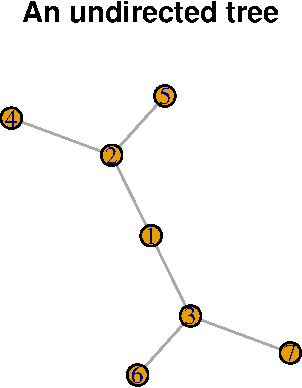
\includegraphics[width=0.45\textwidth]{FIGS/graphs-make-trees-1.pdf}
\quad
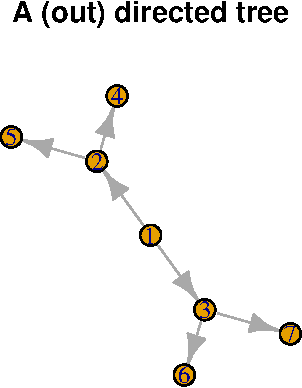
\includegraphics[width=0.45\textwidth]{FIGS/graphs-make-trees-2.pdf}
\end{center}
\end{frame}


\begin{frame}
	\begin{property}
	\begin{itemize}
	\item Every edge of a tree is a bridge
	\item Given two vertices $u $ and $v$ of a tree, there is an unique path linking $u$ to $v$
	\item A tree with $p$ vertices and $q$ edges satisfies $q=p-1$. Thus, a tree is minimally connected
	\end{itemize}
	\end{property}
	\vfill
	(First property: the deletion of any edge of a tree diconnects it)
\end{frame}

\begin{frame}[fragile]\frametitle{Every edge of a tree is a bridge}
\begin{knitrout}
\definecolor{shadecolor}{rgb}{0.969, 0.969, 0.969}\color{fgcolor}\begin{kframe}
\begin{alltt}
\hlkwd{E}\hldef{(G_tu)}
\end{alltt}
\begin{verbatim}
## + 6/6 edges from 51d56f2:
## [1] 1--2 1--3 2--4 2--5 3--6 3--7
\end{verbatim}
\begin{alltt}
\hlkwd{bridges}\hldef{(G_tu)}
\end{alltt}
\begin{verbatim}
## + 6/6 edges from 51d56f2:
## [1] 2--4 2--5 1--2 3--6 3--7 1--3
\end{verbatim}
\begin{alltt}
\hlkwd{all}\hldef{(}\hlkwd{sort}\hldef{(}\hlkwd{E}\hldef{(G_tu))} \hlopt{==} \hlkwd{sort}\hldef{(}\hlkwd{bridges}\hldef{(G_tu)))}
\end{alltt}
\begin{verbatim}
## [1] TRUE
\end{verbatim}
\end{kframe}
\end{knitrout}
\end{frame}


\begin{frame}\frametitle{Spanning tree}
	\begin{definition}[Spanning tree]
	A \defword{spanning tree} of a connected graph $G$ is a subgraph of $G$ that contains all the vertices of $G$ and is a tree.
	\end{definition}
	\vfill
	A graph may have many spanning trees
\end{frame}


\begin{frame}\frametitle{Minimal spanning tree}
	\begin{definition}[{Value of a spanning tree}]
	The \defword{value of a spanning tree} $T$ of order $p$ is
	$$\sum_{i=1}^{p-1}f(e_i)$$
	where $f$ is the function that maps the edge set into $\IR$
	\end{definition}
	\vfill
	\begin{definition}[{Minimal spanning tree}]
	Let $G$ be an undirected network, and let $T$ be a \defword{minimal spanning tree} of $G$. Then $T$ is a spanning tree whose the value is minimum
	\end{definition}
\end{frame}

\begin{frame}\frametitle{Algorithm to find a minimal spanning tree}
Let $G=(V(G),E(G))$ be an undirected network and $T$ be a minimal spanning tree 
\vfill
\begin{enumerate}
\item Sort the edges of $G$ in increasing order by value
\item $T=(V(G),\emptyset)$
\item For each edge $e$ in sorted order
        if the endpoints of $e$ are disconnected in $T$
        add $e$ to $T$
\end{enumerate}
\end{frame}


\begin{frame}[fragile]\frametitle{Finding a minimal spanning tree of the Karate graph}
The function \code{mst} finds minimal spanning trees, using distances if no edge weights are provided
\begin{knitrout}
\definecolor{shadecolor}{rgb}{0.969, 0.969, 0.969}\color{fgcolor}\begin{kframe}
\begin{alltt}
\hldef{G_mst} \hlkwb{=} \hlkwd{mst}\hldef{(G)}
\end{alltt}
\end{kframe}
\end{knitrout}
\end{frame}

\maxFrameImage{FIGS/graphs-minimal-spanning-tree-Karate-graph-1.pdf}

\begin{frame}\frametitle{Minimal connector problem}
\begin{itemize}
\item Model: a graph $G$ such that edges represent all possible connections, and each edge has a positive value which represents its cost; 
an undirected network $G$
\item Solution: a  minimal spanning tree $T$ of $G$
\begin{itemize}
\item a spanning tree of $G$ is a subgraph of $G$ that contains all the vertices of $G$ and is a tree.
\item the cost of the spanning tree is the sum of values of the edges of $T$
\item a spanning tree such that no other spanning tree has a smaller cost is a minimmal spanning tree.
\end{itemize}
\end{itemize}
\end{frame}



\begin{frame}
\begin{theorem}[Characterisation of trees]\label{th:characterisation_tree}
$H=(V,U)$ a graph of order $|V|=n>2$. The following are equivalent and all characterise a tree :
\begin{enumerate}
\item $H$ connected and has no cycles
\item $H$ has $n-1$ arcs and no cycles
\item $H$ connected and has exactly $n-1$ arcs
\item $H$ has no cycles, and if an arc is added to $H$, exactly one cycle is created
\item $H$ connected, and if any arc is removed, the remaining graph is not
connected
\item Every pair of vertices of $H$ is connected by one and only one chain
\end{enumerate}
\end{theorem}
\end{frame}



\begin{frame}
\begin{definition}[Pendant vertex]
A vertex is \defword{pendant} if it is adjacent to exactly one other vertex
\end{definition}
\vfill
\begin{theorem}
A tree of order $n\geq 2$ has at least two pendant vertices
\end{theorem}
\end{frame}

\begin{frame}
\begin{theorem}\label{th:partial_graph_tree_G_connected}
A graph $G=(V,U)$ has a partial graph that is a tree $\iff$ $G$ connected
\end{theorem}
\vfill
Recall that a partial graph is a graph generated by a subset of the arcs (Definition~\ref{def:partial_graph} slide~\pageref{def:partial_graph})
\end{frame}

\begin{frame}{Spanning tree}
The procedure in the proof of Theorem~\ref{th:partial_graph_tree_G_connected} gives a \defword{spanning tree}
\vfill
Can also build a spanning tree as follows:
\begin{itemize}
\item Consider any arc $u_0$
\item Find arc $u_1$ that does not form a cycle with $u_0$
\item Find arc $u_2$ that does not form a cycle with $\{u_0,u_1\}$
\item Continue
\item When you cannot continue anymore, you have a spanning tree
\end{itemize}
\end{frame}




\begin{frame}
\begin{theorem}
$G$ connected graph with $\geq 1$ arc. TFAE
\begin{enumerate}
\item $G$ strongly connected
\item Every arc lies on a circuit
\item $G$ contains no cocircuits
\end{enumerate}
\end{theorem}
\end{frame}


\begin{frame}
\begin{theorem}
$G$ graph with $\geq 1$ arc. TFAE
\begin{enumerate}
\item $G$ is a graph without circuits
\item Each arc is contained in a cocircuit
\end{enumerate}
\end{theorem}
\vfill
\begin{theorem}
If $G$ is a strongly connected graph of order $n$, then $G$ has a cycle basis of $\nu(G)$ circuits
\end{theorem}
\end{frame}

\begin{frame}
\begin{definition}[Node, anti-node, branch]
$G=(V,U)$ strongly connected without loops and $>1$ vertex. For each $x\in V$, there is a path from it and a path to it so $x$ has at least 2 incident arcs. Specifically,
\begin{itemize}
\item $x\in V$ with $>2$ incident arcs is a \defword{node}
\item $x\in V$ with $2$ incident arcs is an \defword{anti-node}
\end{itemize}
A path whose only nodes are its endpoints is a \defword{branch}
\end{definition}
\end{frame}

\begin{frame}
\begin{definition}[Minimally connected graph]
$G$ is \defword{minimally connected} if it is strongly connected and removal of any arc destroys strong-connectedness
\end{definition}
A minimally connected graph is 1-graph without loops
\vfill
\begin{definition}[Contraction]
$G=(V,U)$. The \defword{contraction} of the set $A\subset V$ of vertices consists in replacing $A$ by a single vertex $a$ and replacing each arc into (resp. out of) $A$ by an arc with same index into (resp. out of) $a$
\end{definition}
\end{frame}


\begin{frame}
\begin{theorem}
$G$ minimally connected, $A\subset V$ generating a strongly connected subgraph of $G$. Then the contraction of $A$ gives a minimally connected graph
\end{theorem}
\end{frame}

\begin{frame} 
\begin{theorem}
$G$ a minimally connected graph, $G'$ be the minimally connected graph obtained by the contraction of an elementary circuit of $G$.	Then
\[
\nu(G)=\nu(G')+1
\]
\end{theorem}
\vfill
\begin{theorem}
$G$ minimally connected of order $n\geq 2$ $\implies$ $G$ has $\geq 2$ anti-nodes
\end{theorem}
\vfill
\begin{theorem}
$G=(V,U)$. Then the graph $C'$ obtained by contracting each strongly connected component of $G$ contains no circuits
\end{theorem}
\end{frame}


\begin{frame}{Arborescences}
\begin{definition}[Root]
Vertex $a\in V$ in $G=(V,U)$ is a \defword{root} if all vertices of $G$ can be reached by paths \emph{starting} from $a$
\end{definition}
Not all graphs have roots
\vfill
\begin{definition}[Quasi-strong connectedness]
$G$ is \defword{quasi-strongly connected} if $\forall x,y\in V$, exists $z\in V$ (denoted $z(x,y)$ to emphasize dependence on $x,y$) from which there is a path to $x$ and a path to $y$
\end{definition}
Strongly connected $\implies$ quasi-strongly connected (take $z(x,y)=x$); converse not true

Quasi-strongly connected $\implies$ connected
\end{frame}

\begin{frame}{Arborescence}
\begin{definition}[Arborescence]
An \defword{arborescence} is a tree that has a root
\end{definition}
\vfill
\begin{lemma}
$G=(V,U)$ has a root $\iff$ $G$ quasi-strongly connected
\end{lemma}
\end{frame}

\begin{frame}
\begin{theorem}
$H$ graph of order $n>1$. TFAE (and all characterise an arborescence)
\begin{enumerate}
\item $H$ quasi-strongly connected without cycles
\item $H$ quasi-strongly connected with $n-1$ arcs
\item $H$ tree having a root $a$
\item $\exists a\in V$ s.t. all other vertices are connected with $a$ by 1 and only 1 path from $a$
\item $H$ quasi-strongly connected and loses quasi-strong connectedness if any arc is removed
\item $H$ quasi-strongly connected and $\exists a\in V$ s.t.
\begin{align*}
d_H^-(a)&=0 \\
d_H^-(x)&=1\qquad \forall x\neq a
\end{align*}
\item $H$ has no cycles and $\exists a\in V$ s.t.
\begin{align*}
d_H^-(a)&=0 \\
d_H^-(x)&=1\qquad \forall x\neq a
\end{align*}
\end{enumerate}
\end{theorem}
\end{frame}


\begin{frame}
\begin{theorem}
$G$ has a partial graph that is an arborescence $\iff$ $G$ quasi-strongly connected
\end{theorem}
\vfill
\begin{theorem}
$G=(V,E)$ simple connected graph and $x_1\in V$. It is possible to direct all edges of $E$ so that the resulting graph $G_0=(V,U)$ has a spanning tree $H$ s.t.
\begin{enumerate}
	\item $H$ is an arborescence with root $x_1$
	\item The cycles associated with $H$ are circuits
	\item The only elementary circuits of $G_0$ are the cycles associated with $H$
\end{enumerate}
\end{theorem}
\end{frame}


\begin{frame}{Counting trees}
\begin{proposition}
$X$ a set with $n$ distinct objects, $n_1,\ldots,n_p$ nonnegative integers s.t. $n_1+\cdots+n_p=n$. The number of ways to place the $n$ objects into $p$ boxes $X_1,\ldots,X_p$ containing $n_1,\ldots,n_p$ objects respectively is 
\[
	\begin{pmatrix}
		n\\ n_1,\ldots,n_p
	\end{pmatrix}
	=
	\frac{n!}{n_1!\cdots n_p!}
\]
\end{proposition}
\vfill
\begin{proposition}[Multinomial formula]
Let $a_1,\ldots,a_p\in\IR$ be $p$ real numbers, then
\[
	(a_1+\cdots+a_p)^n= 
	\sum_{n_1,\ldots,n_p\geq 0}
	\begin{pmatrix}
		n\\ n_1,\ldots,n_p
	\end{pmatrix}
	(a_1)^{n_1}\cdots(a_p)^{n_p}	
\]
\end{proposition}
\end{frame}


\begin{frame} 
\begin{theorem}
Denote $T(n;d_1,\ldots,d_n)$ the number of distinct trees $H$ with vertices $x_1,\ldots,x_n$ and with degrees $d_H(x_1)=d_1,\ldots,d_H(x_n)=d_n$. Then
\[
	T(n;d_1,\ldots,d_n) = 
	\begin{pmatrix}
		n-2 \\
		d_1-1,\ldots,d_n-1
	\end{pmatrix}
\]
\end{theorem}
\vfill
\begin{theorem}
The number of different trees with vertices $x_1,\ldots,x_n$ is 
$n^{n-2}$
\end{theorem}
\vfill
There is a whole industry of similar results (as well as for arborescences), but we will stop here. The main point is that we are talking about a large number of possibilities..
\end{frame}



%%%%%%%%%%%%%%%%%%%%%%%%
%%%%%%%%%%%%%%%%%%%%%%%%
%%%%%%%%%%%%%%%%%%%%%%%%
%%%%%%%%%%%%%%%%%%%%%%%%
% \section{Index of terms used}
% \begin{frame}{Index}
% 	\printindex
% \end{frame}

\end{document}
